\section{绝热与非绝热表象}
\subsection{绝热近似}\label{sec:jrjs}
在章节\ref{sec:bo}中，我们把体系的总哈密顿量$\hat{H}$分解成核部分$\hat{T}_{\rm nuc}$与电子部分$\hat{H}_{\rm el}$ [Eq.\eqref{eq:hamiltonian_bo}]：
\[\hat{T}_{\rm nuc}=-\sum_{I=1}^M\frac{1}{2M_I}\nabla^2_{\mathbf{R},I},\quad \hat{H}_{\rm el}=-\sum_{i=1}^N\frac{1}{2}\nabla^2_{\mathbf{r},i}+\sum_{I=1}^{M}\sum_{J>I}^{M}\frac{Z_{I}Z_{J}}{|\mathbf{R}_{I}-\mathbf{R}_{J}|}-\sum_{i=1}^{N}\sum_{I=1}^{M}\frac{Z_{I}}{|\mathbf{r}_{i}-\mathbf{R}_{I}|}+\sum_{i=1}^{N}\sum_{j>i}^{N}\frac{1}{|\mathbf{r}_{i}-\mathbf{r}_{j}|}\]
考虑电子本征方程$\hat{H}_{\rm el}\psi(\mathbf{r};\mathbf{R})=E_{\rm el}(R)\psi(\mathbf{r};\mathbf{R})$，考虑有限个电子的系统，其本征态满足：
\[\hat{H}_{\rm el}\psi_n(\mathbf{r};\mathbf{R})=E_n(\mathbf{R})\psi_n(\mathbf{r};\mathbf{R})\]
这里$\psi_n(\mathbf{r};\mathbf{R})$称为绝热电子波函数，$E_n(\mathbf{R})$就是对应的绝热势能面（PES）。由于$\{\psi_n(\mathbf{r};\mathbf{R})\}$在电子坐标空间中构成一组完备标准正交基，由完备性假设，体系总波函数可以展开为电子波函数和核波函数直积的线性组合：
\[\Psi(\mathbf{r},\mathbf{R})=\sum_n\psi_n(\mathbf{r};\mathbf{R})\chi_n(\mathbf{R})\]
其中$\chi_n(\mathbf{R})$是对应第$n$个绝热势能面的核波函数。对整体薛定谔方程乘上$\psi_m^{\dagger}(\mathbf{r};\mathbf{R})$并对电子坐标积分：
\begin{equation}\label{eq:bo_eom}
\begin{aligned}
0=\int\psi_m^{\dagger}(\mathbf{r};\mathbf{R})\left(\hat{H}-E\right)\Psi(\mathbf{R},\mathbf{r})\dd{\mathbf{r}}
&=\sum_n\int\psi_m^{\dagger}(\mathbf{r};\mathbf{R})\left(\hat{T}_{\rm nuc}+\hat{H}_{\rm el}-E\right)\psi_n(\mathbf{r};\mathbf{R})\chi_n(\mathbf{R})\dd{\mathbf{r}}\\
&=\sum_n\int\psi_m^{\dagger}(\mathbf{r};\mathbf{R})\left(\hat{T}_{\rm nuc}+E_n-E\right)\psi_n(\mathbf{r};\mathbf{R})\chi_n(\mathbf{R})\dd{\mathbf{r}}\\
\end{aligned}
\end{equation}
由于电子波函数也包含核坐标，展开$\hat{T}_{\rm nuc}\psi_n(\mathbf{r};\mathbf{R})\chi_n(\mathbf{R})$，注意下面求和中的脚标$I$是代表不同核坐标：
\[-\sum_I\frac{1}{2M_I}\left[\nabla_{\mathbf{R},I}^2\psi_n(\mathbf{r};\mathbf{R})\cdot\chi_n(\mathbf{R})+2\nabla_{\mathbf{R},I}\psi_n(\mathbf{r};\mathbf{R})\cdot\nabla_{\mathbf{R},I}\chi_n(\mathbf{R})+\psi_n(\mathbf{r};\mathbf{R})\cdot\nabla^2_{\mathbf{R},I}\chi_n(\mathbf{R})\right]\]
定义对核波函数$\chi_n(\mathbf{R})$的算符$\hat{\Lambda}_{mn}$：
\begin{equation}\label{eq:na_coupling}
\hat{\Lambda}_{mn}=-\sum_I\frac{1}{2M_I}\left[\left(\int\psi_m^{\dagger}(\mathbf{r};\mathbf{R})\nabla_{\mathbf{R},I}^2\psi_n(\mathbf{r};\mathbf{R})\dd{\mathbf{r}}\right)+2\left(\int\psi_m^{\dagger}(\mathbf{r};\mathbf{R})\nabla_{\mathbf{R},I}\psi_n(\mathbf{r};\mathbf{R})\dd{\mathbf{r}}\right)\nabla_{\mathbf{R},I}\right]
\end{equation}
把上述算符$\hat{\Lambda}_{mn}$带回方程 Eq.\eqref{eq:bo_eom}：
\begin{equation}\label{eq:bh_expansion}
\int\psi_m^{\dagger}(\mathbf{r};\mathbf{R})\left(\hat{H}-E\right)\Psi(\mathbf{R},\mathbf{r})\dd{\mathbf{r}}
=\left(\hat{T}_{\rm nuc}+E_m-E\right)\chi_m(\mathbf{R})+\sum_n\hat{\Lambda}_{mn}\chi_n(\mathbf{R})=0
\end{equation}

上述用绝热电子波函数展开整体波函数的方法称为 Born-Huang 展开，由 Max Born 和 Kun Huang（黄昆）最早提出。回顾章节\ref{sec:bo}中提及的的 BO 近似，\textcolor{blue}{\textbf{其本质并不是简单地把核钉住不动，而是忽略核动能诱导的电子态间耦合}}。在最粗糙的 BO 近似下，我们直接舍去全部$\hat{\Lambda}_{mn}$，于是每一张势能面上的核方程彼此解耦：
\[\left(\hat{T}_{\rm nuc}+E_m-E\right)\chi_m(\mathbf{R})=0 \quad \Leftrightarrow \quad \left(\hat{T}_{\rm nuc}+E_m\right)\chi_m(\mathbf{R})=E\chi_m(\mathbf{R})\]
如果只保留对角项$\hat{\Lambda}_{mm}$而忽略非对角项$\hat{\Lambda}_{mn}, \ (m \neq n)$，则得到比最简单 BO 近似更精细的绝热核方程：
\[\left(\hat{T}_{\rm nuc}+E_m-E\right)\chi_m(\mathbf{R})+\hat{\Lambda}_{mm}\chi_m(\mathbf{R})=0 \quad \Leftrightarrow \quad \left(\hat{T}_{\rm nuc}+E_m+\hat{\Lambda}_{mm}\right)\chi_m(\mathbf{R})=E\chi_m(\mathbf{R})\]
而真正导致电子态之间跃迁的，正是这些非对角的非绝热耦合项。绝热近似和 BO 近似的一个重要差别是：\textcolor{blue}{\textbf{BO 近似中核感受到的有效势$E_m$完全来自于电子部分的贡献，不包含包含核质量的影响（而耦合算符$\hat{\Lambda}_{mm}$中包含核质量），因此无法区分同位素}}。绝热近似本质上是忽略不同电子态的耦合，在考虑原子核运动时假定电子始终处在基态。当体系处在平衡结构附近时，不同电子态之间的能量差一般都显著大于原子核运动(振动，转动，平动)对应的能量，但是在涉及化学键形成或断裂的反应动力学过程中，电子基态和激发态能量有可能会非常接近甚至出现简并的情形，这时就必须考虑不同电子态之间的耦合。与不同电子态耦合有关的物理效应被称非绝热效应(nonadiabatic effects)，相应的动力学称为非绝热动力学(non-adiabatic dynamics).

\newpage
\subsection{非绝热耦合与绝热表象}
从上一小节中定义的耦合算符$\hat{\Lambda}_{mn}$出发，定义一阶与二阶导数耦合矩阵元：
\[\mathbf{F}^I_{mn}(\mathbf{R})=\int\psi_m^{\dagger}(\mathbf{r};\mathbf{R})\nabla_{\mathbf{R},I}\psi_n(\mathbf{r};\mathbf{R})\dd{\mathbf{r}}, \quad \mathbf{G}^I_{mn}(\mathbf{R})=\int\psi_m^{\dagger}(\mathbf{r};\mathbf{R})\nabla_{\mathbf{R},I}^2\psi_n(\mathbf{r};\mathbf{R})\dd{\mathbf{r}}\]
则上一小节中的耦合算符$\hat{\Lambda}_{mn}$ [Eq.\eqref{eq:na_coupling}]可以改写为：
\[\hat{\Lambda}_{mn}=-\sum_I\frac{1}{2M_I}\left[2\mathbf{F}^I_{mn}(\mathbf{R})\nabla_{\mathbf{R},I}+\mathbf{G}^I_{mn}(\mathbf{R})\right]\]
将上式带回 Born-Huang 展开得到的耦合核方程 [Eq.\eqref{eq:bo_eom}]，并展开可得：
\[\begin{aligned}
\left[-\sum_I\frac{1}{2M_I}\nabla^2_{\mathbf{R},I}+E_m(\mathbf{R})-E\right]\chi_m(\mathbf{R})-\sum_I\frac{1}{2M_I}\sum_n\left[2\mathbf{F}^I_{mn}(\mathbf{R})\nabla_{\mathbf{R},I}+\mathbf{G}^I_{mn}(\mathbf{R})\right]\chi_n(\mathbf{R})&=0\\
\sum_n\left\{-\sum_I\frac{1}{2M_I}\left[\delta_{mn}\nabla^2_{\mathbf{R},I}+2\mathbf{F}^I_{mn}(\mathbf{R})\nabla_{\mathbf{R},I}+\mathbf{G}^I_{mn}(\mathbf{R})\right]+\left[E_n(\mathbf{R})-E\right]\delta_{mn}\right\}\chi_n(\mathbf{R})&=0
\end{aligned}\]
将上述方程写成矩阵形式，令$\bm{\chi}^{(a)}(\mathbf{R})$为核波函数向量，$\mathbf{V}^{(a)}_{mn}(\mathbf{R})=E_n(\mathbf{R})\delta_{mn}$为绝热势能矩阵矩阵元，并记由$\mathbf{F}^{I}_{mn}(\mathbf{R})$与$\mathbf{G}^{I}_{mn}(\mathbf{R})$组成的矩阵分别为$\mathbf{F}^{I}(\mathbf{R})$与$\mathbf{G}^{I}(\mathbf{R})$，
则上式可写成绝热表象下的矩阵形式：
\begin{equation}\label{eq:a_eom}
\left[-\sum_I\frac{1}{2M_I}\left(\nabla_{\mathbf{R},I}^2\mathbbm{1}+2\mathbf{F}^{I}(\mathbf{R})\nabla_{\mathbf{R},I}+\mathbf{G}^{I}(\mathbf{R})\right)+\mathbf{V}^{(a)}(\mathbf{R})-E\mathbbm{1}\right]\bm{\chi}^{(a)}(\mathbf{R})=0
\end{equation}

上述方程 Eq.\eqref{eq:a_eom}即为绝热表象下的精确核薛定谔方程。可以看到，\textcolor{blue}{\textbf{在绝热表象里势能矩阵$\mathbf{V}^{(a)}(\mathbf{R})$仍然是对角的，但所有的耦合项都包含在动能项中，处理起来还是异常麻烦。}}另一方面，方程 Eq.\eqref{eq:a_eom} 中很难直接看出一个动能项，但是我们做一些推导使得其形式上与正常薛定谔方程相近。从电子波函数的正交归一性出发：
\[\delta_{mn}=\int\psi_m^{\dagger}(\mathbf{r};\mathbf{R})\psi_n(\mathbf{r};\mathbf{R})\dd{\mathbf{r}} \ \Rightarrow \ \nabla_{\mathbf{R},I}\delta_{mn}=\int\left[(\nabla_{\mathbf{R},I}\psi_m(\mathbf{r};\mathbf{R}))^{\dagger}\psi_n(\mathbf{r};\mathbf{R})+\psi_m^{\dagger}(\mathbf{r};\mathbf{R})\nabla_{\mathbf{R},I}\psi_n(\mathbf{r};\mathbf{R})\right]\dd{\mathbf{r}}=0\]
容易看出$\mathbf{F}_{mn}^I(\mathbf{R})=-\left(\mathbf{F}_{nm}^I(\mathbf{R})\right)^*$，即一阶导数耦合矩阵$\mathbf{F}^I$都是反厄米的。对$\mathbf{F}_{mn}^I$再求导：
\begin{equation}\label{eq:hds}
\begin{aligned}
\nabla_{\mathbf{R},I}\mathbf{F}_{mn}^I&=\int(\nabla_{\mathbf{R},I}\psi_m(\mathbf{r};\mathbf{R}))^{\dagger}\cdot\nabla_{\mathbf{R},I}\psi_n(\mathbf{r};\mathbf{R})\dd{\mathbf{r}}+\int\psi_m^{\dagger}(\mathbf{r};\mathbf{R})\nabla_{\mathbf{R},I}^2\psi_n(\mathbf{r};\mathbf{R})\dd{\mathbf{r}}\\
&=\iint(\nabla_{\mathbf{R},I}\psi_m(\mathbf{r};\mathbf{R}))^{\dagger}\delta(\mathbf{r}-\mathbf{r}')\nabla_{\mathbf{R},I}\psi_n(\mathbf{r}';\mathbf{R})\dd{\mathbf{r}}\dd{\mathbf{r}'}+\mathbf{G}_{mn}^I\\
&=\sum_k\iint(\nabla_{\mathbf{R},I}\psi_m(\mathbf{r};\mathbf{R}))^{\dagger}\psi_k(\mathbf{r};\mathbf{R})\psi_k^{\dagger}(\mathbf{r}';\mathbf{R})\nabla_{\mathbf{R},I}\psi_n(\mathbf{r}';\mathbf{R})\dd{\mathbf{r}}\dd{\mathbf{r}'}+\mathbf{G}_{mn}^I\\
&=\sum_k\left[\int(\nabla_{\mathbf{R},I}\psi_m(\mathbf{r};\mathbf{R}))^{\dagger}\psi_k(\mathbf{r};\mathbf{R})\dd{\mathbf{r}}\right]\cdot\left[\int\psi_k^{\dagger}(\mathbf{r}';\mathbf{R})\nabla_{\mathbf{R},I}\psi_n(\mathbf{r}';\mathbf{R})\dd{\mathbf{r}'}\right]+\mathbf{G}_{mn}^I\\
&=-\sum_k\mathbf{F}_{mk}^I\mathbf{F}_{kn}^I+\mathbf{G}_{mn}^I
\end{aligned}
\end{equation}
这里严格的做法是先插入$\delta(\mathbf{r}-\mathbf{r}')$引入第二个电子坐标$\mathbf{r}'$，再利用完备性关系：
\[\boxed{\delta(\mathbf{r}-\mathbf{r}')=\sum_k\psi_k(\mathbf{r};\mathbf{R})\psi_k^{\dagger}(\mathbf{r}';\mathbf{R})}\]
把它展开。我们定一个带修正带核动能算符(dressed kinetic energy operator，我也不知道怎么翻译)：
\[\left[\left(\nabla_{\mathbf{R},I}+\mathbf{F}^I\right)^2\right]_{mn}=\delta_{mn}\nabla_{\mathbf{R},I}^2+\mathbf{F}_{mn}^I\nabla_{\mathbf{R},I}+\nabla_{\mathbf{R},I}\mathbf{F}_{mn}^I+\sum_k\mathbf{F}_{mk}^I\mathbf{F}_{kn}^I=\delta_{mn}\nabla_{\mathbf{R},I}^2+2\mathbf{F}_{mn}^I\nabla_{\mathbf{R},I}+G_{mn}^I\]
上式的系数$2$的来源参考$\nabla(fg)=f\nabla g+g\nabla f$，这里令$g$是核波函数。因此方程 Eq.\eqref{eq:a_eom} 可以进一步改写为：
\begin{equation}
\left[-\sum_I\frac{1}{2M_I}\left(\nabla_{\mathbf{R},I}+\mathbf{F}^I(\mathbf{R})\right)^2+\mathbf{V}^{(a)}(\mathbf{R})-E\mathbbm{1}\right]\bm{\chi}^{(a)}(\mathbf{R})=0
\end{equation}

至此我们可以稍作总结，\textcolor{blue}{\textbf{绝热表象的好处是势能面仍然保持对角，但代价是核动能项不再是朴素的拉普拉斯算符}}。这里稍微解释一下为什么不用狄拉克符号来做本章的推导，因为在狄拉克符号下坐标的归属不明确，上述利用$\delta(\mathbf{r}-\mathbf{r}')$进行的计算在狄拉克符号下不能体现。你不会想写$\ket{\psi_m(\mathbf{r};\mathbf{R})}$吧？

一般来说实际计算里通常不会保留全部电子态，而只保留一组彼此接近、耦合显著的绝热态，记作$g$。则在这个截断子空间中，核方程写成：
\[\sum_{n\in g}\left[-\sum_I\frac{1}{2M_I}\left[\left(\nabla_{\mathbf{R},I}+\mathbf{F}^{I,(g)}(\mathbf{R})\right)^2\right]_{mn}+E_n(\mathbf{R})\delta_{mn}-E\delta_{mn}\right]\chi_n^{(g)}(\mathbf{R})=0\]
那些被扔到子空间外的那些态的影响可以近似描述为一种修正势，即将势能矩阵$E_n(\mathbf{R})\delta_{mn}$修正为：
\[\mathbf{V}_{mn}^{(g)}(\mathbf{R})=E_n(\mathbf{R})\delta_{mn}+\sum_I\frac{1}{2M_I}\int\left(\nabla_{\mathbf{R},I}\psi_m(\mathbf{r};\mathbf{R})\right)^{\dagger}\left(1-\hat{P}_g\right)\nabla_{\mathbf{R},I}\psi_n(\mathbf{r};\mathbf{R})\dd{\mathbf{r}}\]
其中$\hat{P}_g$是选取的核波函数子空间$g$的投影算符。

采用非绝热表象还有一个坏处是非绝热耦合在圆锥交叉附近有奇异性。从电子本征方程出发：
\[\hat{H}_{\rm el}\psi_n(\mathbf{r};\mathbf{R})=E_n(\mathbf{R})\psi_n(\mathbf{r};\mathbf{R})\]
对方程两侧求导$\nabla_{\mathbf{R},I}$并左乘$\psi_m^{\dagger}$并对电子坐标积分，当$m\neq n$时有：
\[\begin{aligned}
\int\psi_m^{\dagger}(\nabla_{\mathbf{R},I}\hat{H}_{\rm el})\psi_n\dd{\mathbf{r}}+\int\psi_m^{\dagger}\hat{H}_{\rm el}\nabla_{\mathbf{R},I}\psi_n\dd{\mathbf{r}}&=\nabla_{\mathbf{R},I}E_n\int\psi_m^{\dagger}\psi_n\dd{\mathbf{r}}+E_n\int\psi_m^{\dagger}\nabla_{\mathbf{R},I}\psi_n\dd{\mathbf{r}}\\
\int\psi_m^{\dagger}(\nabla_{\mathbf{R},I}\hat{H}_{\rm el})\psi_n\dd{\mathbf{r}}+E_m\mathbf{F}_{mn}^I&=0+E_n\mathbf{F}_{mn}^I\\
\end{aligned}\]
\[\Rightarrow \quad \mathbf{F}_{mn}^I(\mathbf{R})=\frac{1}{E_n(\mathbf{R})-E_m(\mathbf{R})}\int\psi_m^{\dagger}(\mathbf{r};\mathbf{R})(\nabla_{\mathbf{R},I}\hat{H}_{\rm el})\psi_n(\mathbf{r};\mathbf{R})\dd{\mathbf{r}}\]

显然上式在$E_n(\mathbf{R})-E_m(\mathbf{R})=0$时奇异。这在势能面上体现为在圆锥交叉(conical intersection)处，导数耦合奇异。于是我们就能明白为什么 BO 近似和绝热近似都会在这些区域及其附近都会失效：\textcolor{blue}{\textbf{绝热表象把奇异性留在了导数耦合里，势能面越接近，非绝热跃迁就越不能被忽略}}。

\subsection{透热表象}
绝热表象只是按照能量大小对势能面进行机械的排序，且由于不同势能面解耦，势能面$E_n^{(a)}(\mathbf{R})$直接彼此不交叉（下图不同分支），上一小节提及了绝热表象下核波函数对应的动能项不是简单的拉普拉斯算符，那么我们自然而然的会想能否有一种表现可以保留简单的动能项呢？有的兄弟，有的。这就是透热表象(diabatic representation)，我们通过对绝热表象做一个酉变换获得有简单动能项的透热表象，把复杂的耦合留给势能项。之所以得名透热，是因为透热势能面（下图相同颜色）之间可以彼此交叉。

\begin{center}
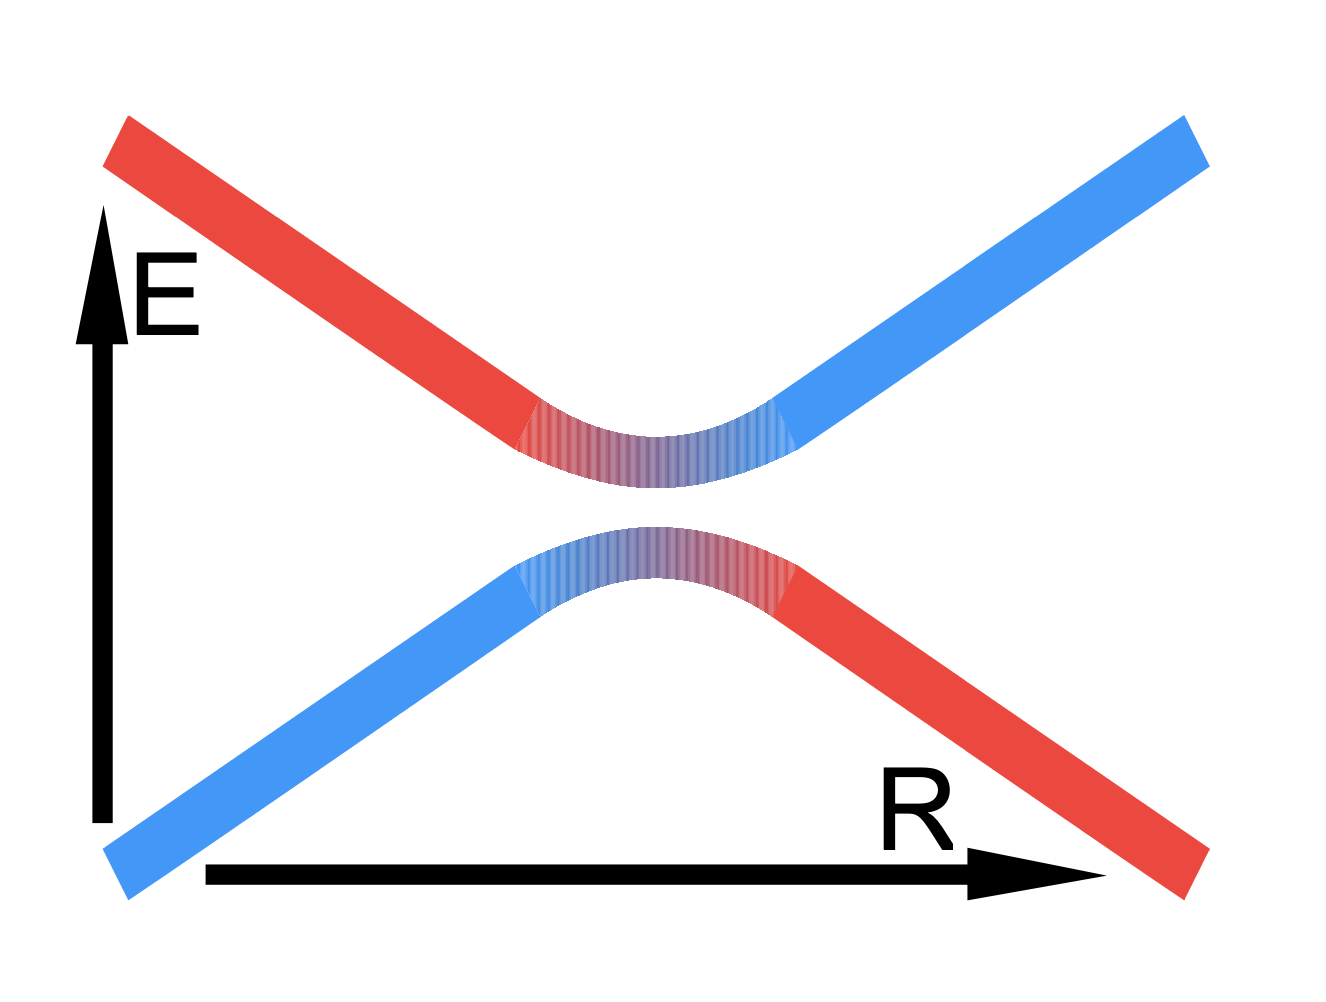
\includegraphics[width=0.4\textwidth]{fig/quantum_chemistry/pes.png}
\end{center}

从电子波函数（行向量）和对应的核波函数（列向量）展开的矩阵形式出发：
\[\Psi(\mathbf{r},\mathbf{R})=\sum_n\psi_n(\mathbf{r};\mathbf{R})\chi_n(\mathbf{R}) \quad \Rightarrow \quad \Psi(\mathbf{r},\mathbf{R})=\bm{\psi}^{(a)}(\mathbf{r};\mathbf{R})\bm{\chi}^{(a)}(\mathbf{R})\]
现在取幺正变换$\mathbf{U}(\mathbf{R})$，满足$\mathbf{U}^{\dagger}(\mathbf{R})\mathbf{U}(\mathbf{R})=\mathbbm{1}$。定义透热电子波函数$\bm{\psi}^{(d)}(\mathbf{r};\mathbf{R})$与核波函数$\bm{\chi}^{(d)}(\mathbf{R})$：
\[\bm{\psi}^{(d)}(\mathbf{r};\mathbf{R})=\bm{\psi}^{(a)}(\mathbf{r};\mathbf{R})\mathbf{U}(\mathbf{R}), \quad \bm{\chi}^{(d)}(\mathbf{R})=\mathbf{U}^{\dagger}(\mathbf{R})\bm{\chi}^{(a)}(\mathbf{R}) \quad \Rightarrow \quad \Psi(\mathbf{r},\mathbf{R})=\bm{\psi}^{(d)}(\mathbf{r};\mathbf{R})\bm{\chi}^{(d)}(\mathbf{R})\]
透热表象只是对电子态子空间做了一个基底变换，总波函数和一切可观测量都不会因此改变。

将$\bm{\chi}^{(a)}(\mathbf{R})=\mathbf{U}(\mathbf{R})\bm{\chi}^{(d)}(\mathbf{R})$代入绝热表象下的精确核方程 [Eq.\eqref{eq:a_eom}]：
\[\left[-\sum_I\frac{1}{2M_I}\left(\nabla_{\mathbf{R},I}^2\mathbbm{1}+2\mathbf{F}^{I}(\mathbf{R})\nabla_{\mathbf{R},I}+\mathbf{G}^{I}(\mathbf{R})\right)+\mathbf{V}^{(a)}(\mathbf{R})-E\mathbbm{1}\right]\mathbf{U}(\mathbf{R})\bm{\chi}^{(d)}(\mathbf{R})=0\]
对核导数逐项展开：
\[\begin{aligned}
\nabla_{\mathbf{R},I}\left(\mathbf{U}\bm{\chi}^{(d)}\right)&=\left(\nabla_{\mathbf{R},I}\mathbf{U}\right)\bm{\chi}^{(d)}+\mathbf{U}\nabla_{\mathbf{R},I}\bm{\chi}^{(d)}\\
\nabla_{\mathbf{R},I}^2\left(\mathbf{U}\bm{\chi}^{(d)}\right)&=\left(\nabla_{\mathbf{R},I}^2\mathbf{U}\right)\bm{\chi}^{(d)}+2\left(\nabla_{\mathbf{R},I}\mathbf{U}\right)\nabla_{\mathbf{R},I}\bm{\chi}^{(d)}+\mathbf{U}\nabla_{\mathbf{R},I}^2\bm{\chi}^{(d)}
\end{aligned}\]
于是绝热表象方程可化为：
\begin{equation}\label{eq:d_emo_temp}
\begin{aligned}
0=&\left[\mathbf{V}^{(a)}(\mathbf{R})-E\mathbbm{1}\right]\mathbf{U}\bm{\chi}^{(d)}-\sum_I\frac{1}{2M_I}\Big[\nabla_{\mathbf{R},I}^2\mathbf{U}+2\mathbf{F}^{I}(\mathbf{R})\nabla_{\mathbf{R},I}\mathbf{U}+\mathbf{G}^{I}(\mathbf{R})\mathbf{U}\Big]\bm{\chi}^{(d)}\\
&-\sum_I\frac{1}{2M_I}\Big[2\nabla_{\mathbf{R},I}\mathbf{U}+2\mathbf{F}^{I}(\mathbf{R})\mathbf{U}\Big]\nabla_{\mathbf{R},I}\bm{\chi}^{(d)}-\sum_I\frac{1}{2M_I}\mathbf{U}\nabla_{\mathbf{R},I}^2\bm{\chi}^{(d)}
\end{aligned}
\end{equation}
为保留动能项为简单拉普拉斯算子，我们要求$\nabla_{\mathbf{R},I}\bm{\chi}^{(d)}$前面的系数为零，即得透热变换矩阵$\mathbf{U}(\mathbf{R})$的约束方程：
\begin{equation}\label{eq:ysfc}
\nabla_{\mathbf{R},I}\mathbf{U}(\mathbf{R})+\mathbf{F}^{I}(\mathbf{R})\mathbf{U}(\mathbf{R})=0
\end{equation}
对限制方程再作用一次$\nabla_{\mathbf{R},I}$：
\begin{equation}\label{eq:nabla_ysfc}
\nabla_{\mathbf{R},I}^2\mathbf{U}+\mathbf{F}^{I}(\mathbf{R})\left[\nabla_{\mathbf{R},I}\mathbf{U}(\mathbf{R})\right]+\left[\nabla_{\mathbf{R},I}\mathbf{F}^{I}(\mathbf{R})\right]\mathbf{U}(\mathbf{R})=0
\end{equation}
由上一小节证明的恒等式 Eq.\eqref{eq:hds}可知：
\[\nabla_{\mathbf{R},I}^2\mathbf{U}+\mathbf{F}^{I}(\mathbf{R})\left[\nabla_{\mathbf{R},I}\mathbf{U}(\mathbf{R})\right]+\left[\mathbf{G}^{I}(\mathbf{R})-\left(\mathbf{F}^{I}(\mathbf{R})\right)^2\right]\mathbf{U}(\mathbf{R})=0\]
展开$\left(\mathbf{F}^{I}(\mathbf{R})\right)^2=\mathbf{F}^{I}(\mathbf{R})\mathbf{F}^{I}(\mathbf{R})$后带入约束方程 [Eq.\eqref{eq:ysfc}] 可将 Eq.\eqref{eq:nabla_ysfc} 整理成：
\[\nabla_{\mathbf{R},I}^2\mathbf{U}+2\mathbf{F}^{I}(\mathbf{R})\nabla_{\mathbf{R},I}\mathbf{U}+\mathbf{G}^{I}(\mathbf{R})\mathbf{U}=0\]
因此方程 Eq.\eqref{eq:d_emo_temp} 中含$\bm{\chi}^{(d)}$的项系数为$0$，最后在方程 Eq.\eqref{eq:d_emo_temp} 左乘一个$\mathbf{U}^{\dagger}(\mathbf{R})$得到透热表象下的核方程：
\[\left[-\sum_I\frac{1}{2M_I}\nabla_{\mathbf{R},I}^2\mathbbm{1}+\mathbf{V}^{(d)}(\mathbf{R})-E\mathbbm{1}\right]\bm{\chi}^{(d)}(\mathbf{R})=0\]
其中：
\begin{equation}\label{eq:potential_transform}
\mathbf{V}^{(d)}(\mathbf{R})=\mathbf{U}^{\dagger}(\mathbf{R})\mathbf{V}^{(a)}(\mathbf{R})\mathbf{U}(\mathbf{R})
\end{equation}
在透热表象中\textcolor{blue}{\textbf{绝热表象里的一阶导数耦合被消去了，但原本对角的势能矩阵变成了非对角矩阵}}。

综上所述，绝热表象和透热表象只是把“耦合”放在了不同的位置。在处理 avoided crossing、电子跃迁以及非绝热动力学时，透热表象往往比绝热表象更方便。另一方面，严格的全局透热基底通常并不容易构造，这也是为什么实际计算里很多时候只能得到局域的 quasi-diabatic 表象。

现在我们再回看透热约束方程 Eq.\eqref{eq:ysfc}，其本质上是一个关于核坐标的矩阵微分方程。沿着核坐标空间中的一条路径$\gamma:\mathbf{R}_0\to\mathbf{R}$，它的形式解可以写成路径有序指数：
\[\mathbf{U}(\mathbf{R})=\mathcal{P}\exp\left[-\int_{\gamma}\sum_I\mathbf{F}^{I}(\mathbf{R}')\cdot\dd{\mathbf{R}'_I}\right]\mathbf{U}(\mathbf{R}_0)\]
这里$\mathcal{P}$表示按路径排序(path ordering)。如果把路径离散成一系列很小的步长$\Delta \mathbf{R}_I$，则可以近似写成：
\[\mathbf{U}(\mathbf{R})\approx\prod_n\exp\left[-\sum_I\mathbf{F}^{I}(\mathbf{R}_n)\cdot\Delta \mathbf{R}_{I,n}\right]\mathbf{U}(\mathbf{R}_0)\]
通常会选一个远离 avoided crossing 的参考构型$\mathbf{R}_0$，并取$\mathbf{U}(\mathbf{R}_0)=\mathbbm{1}$作为初值，然后沿着路径逐步传播到目标构型。这样做的难点不在形式，而在于$\mathbf{F}^{I}(\mathbf{R})$本身往往很难精确计算，而且不同路径得到的结果还可能并不完全一致，这也反映了全局透热表象构造的微妙性。

\newpage
\subsection{电子转移的经典模型：Marcus理论}
作为展示，在这一小节我们考虑最简单的非简并两态模型，则体系哈密顿$\hat{H}$分别可以在绝热表象和透热表象下写成一个$2 \times 2$的矩阵，记两个透热态分别为$\bm{\chi}^{(d)}_1(\mathbf{R})$和$\bm{\chi}^{(d)}_2(\mathbf{R})$，两个绝热态分别为$\bm{\chi}^{(a)}_+(\mathbf{R})$和$\bm{\chi}^{(a)}_-(\mathbf{R})$：
\[\begin{aligned}
\mathbf{H}^{(a)}(\mathbf{R})&=
\begin{pmatrix}
T_{+,\rm{nuc}}(\mathbf{R}) & F_{+-}(\mathbf{R})\\
F_{-+}(\mathbf{R}) & T_{-,\rm{nuc}}(\mathbf{R})
\end{pmatrix}
+
\begin{pmatrix}
E_+(\mathbf{R}) & 0\\
0 & E_-(\mathbf{R})
\end{pmatrix}\\
\mathbf{H}^{(d)}(\mathbf{R})&=\begin{pmatrix}
T_{+,\rm{nuc}}(\mathbf{R}) & 0\\
0 & T_{-,\rm{nuc}}(\mathbf{R})
\end{pmatrix}
+
\begin{pmatrix}
V_{11}^{(d)}(\mathbf{R}) & V_{12}^{(d)}(\mathbf{R})\\
V_{21}^{(d)}(\mathbf{R}) & V_{22}^{(d)}(\mathbf{R})
\end{pmatrix}
\end{aligned}\]
由完备性假设，我们可以用透热态$\bm{\chi}^{(d)}_1(\mathbf{R})$和$\bm{\chi}^{(d)}_2(\mathbf{R})$来展开绝热态$\bm{\chi}^{(a)}_+(\mathbf{R})$和$\bm{\chi}^{(a)}_-(\mathbf{R})$，因此两者之间存在一个幺正变换$\mathbf{U}(\mathbf{R})$，使得$\bm{\chi}^{(a)}(\mathbf{R})=\bm{\chi}^{(d)}(\mathbf{R})\mathbf{U}(\mathbf{R})$，由 Eq.\eqref{eq:potential_transform}可知$\mathbf{U}(\mathbf{R})$可通过对透热势能矩阵对角化获得：
\[
\begin{pmatrix}
\bm{\chi}^{(a)}_+(\mathbf{R}) \\
\bm{\chi}^{(a)}_-(\mathbf{R})
\end{pmatrix}
=
\begin{pmatrix}
\mathbf{U}_{+1}(\mathbf{R}) & \mathbf{U}_{+2}(\mathbf{R}) \\
\mathbf{U}_{-1}(\mathbf{R}) & \mathbf{U}_{-2}(\mathbf{R})
\end{pmatrix}
\begin{pmatrix}
\bm{\chi}^{(d)}_1(\mathbf{R}) \\
\bm{\chi}^{(d)}_2(\mathbf{R})
\end{pmatrix}
\]
不失一般性，设$\Delta V=V_{11}^{(d)}(\mathbf{R})-V_{22}^{(d)}(\mathbf{R})>0$，则$\mathbf{U}$具体表达式如下：
\[\mathbf{U}(\mathbf{R})=\begin{pmatrix}
\cos\gamma & -\sin\gamma\\
\sin\gamma & \cos\gamma
\end{pmatrix}, \quad \gamma=\frac{1}{2}\arctan\left(\frac{2V_{12}^{(d)}(\mathbf{R})}{\Delta V(\mathbf{R})}\right)\]
则容易得到绝热态的势能表达式为：
\[E_{\pm}(\mathbf{R})=\frac{1}{2}\left(V_{11}^{(d)}(\mathbf{R})+V_{22}^{(d)}(\mathbf{R})\pm\sqrt{\left(V_{11}^{(d)}(\mathbf{R})-V_{22}^{(d)}(\mathbf{R})\right)^2+4|V_{12}^{(d)}(\mathbf{R})|^2}\right)\]

透热表象下的势能面$V_{11}^{(d)}(\mathbf{R})$和$V_{22}^{(d)}(\mathbf{R})$因为相互独立所以可以交叉，而绝热表象下的势能面$E_{\pm}(\mathbf{R})$要想交叉，在满足$V_{11}^{(d)}(\mathbf{R})=V_{22}^{(d)}(\mathbf{R})$之外还需耦合$V_{12}^{(d)}(\mathbf{R})=0$，这是不可能达到的，因此绝热势能面不会交叉。另外我可以知道在透热势能面的交叉点处，两绝热势能面的差值为$2|V_{12}^{(d)}(\mathbf{R})|$。假设透热势能面是两个谐振子势（虚线），图\ref{fig:tls_e_c}展示了两种可能的不同形状（单抛物线和双抛物线）的绝热势能面（实线），这两者的差异仅仅取决于两谐振子势的接近程度。上半图中底部的虚线表示绝热势能面与靠近的透热势能面的差值。

\begin{figure}[htbp]
\centering
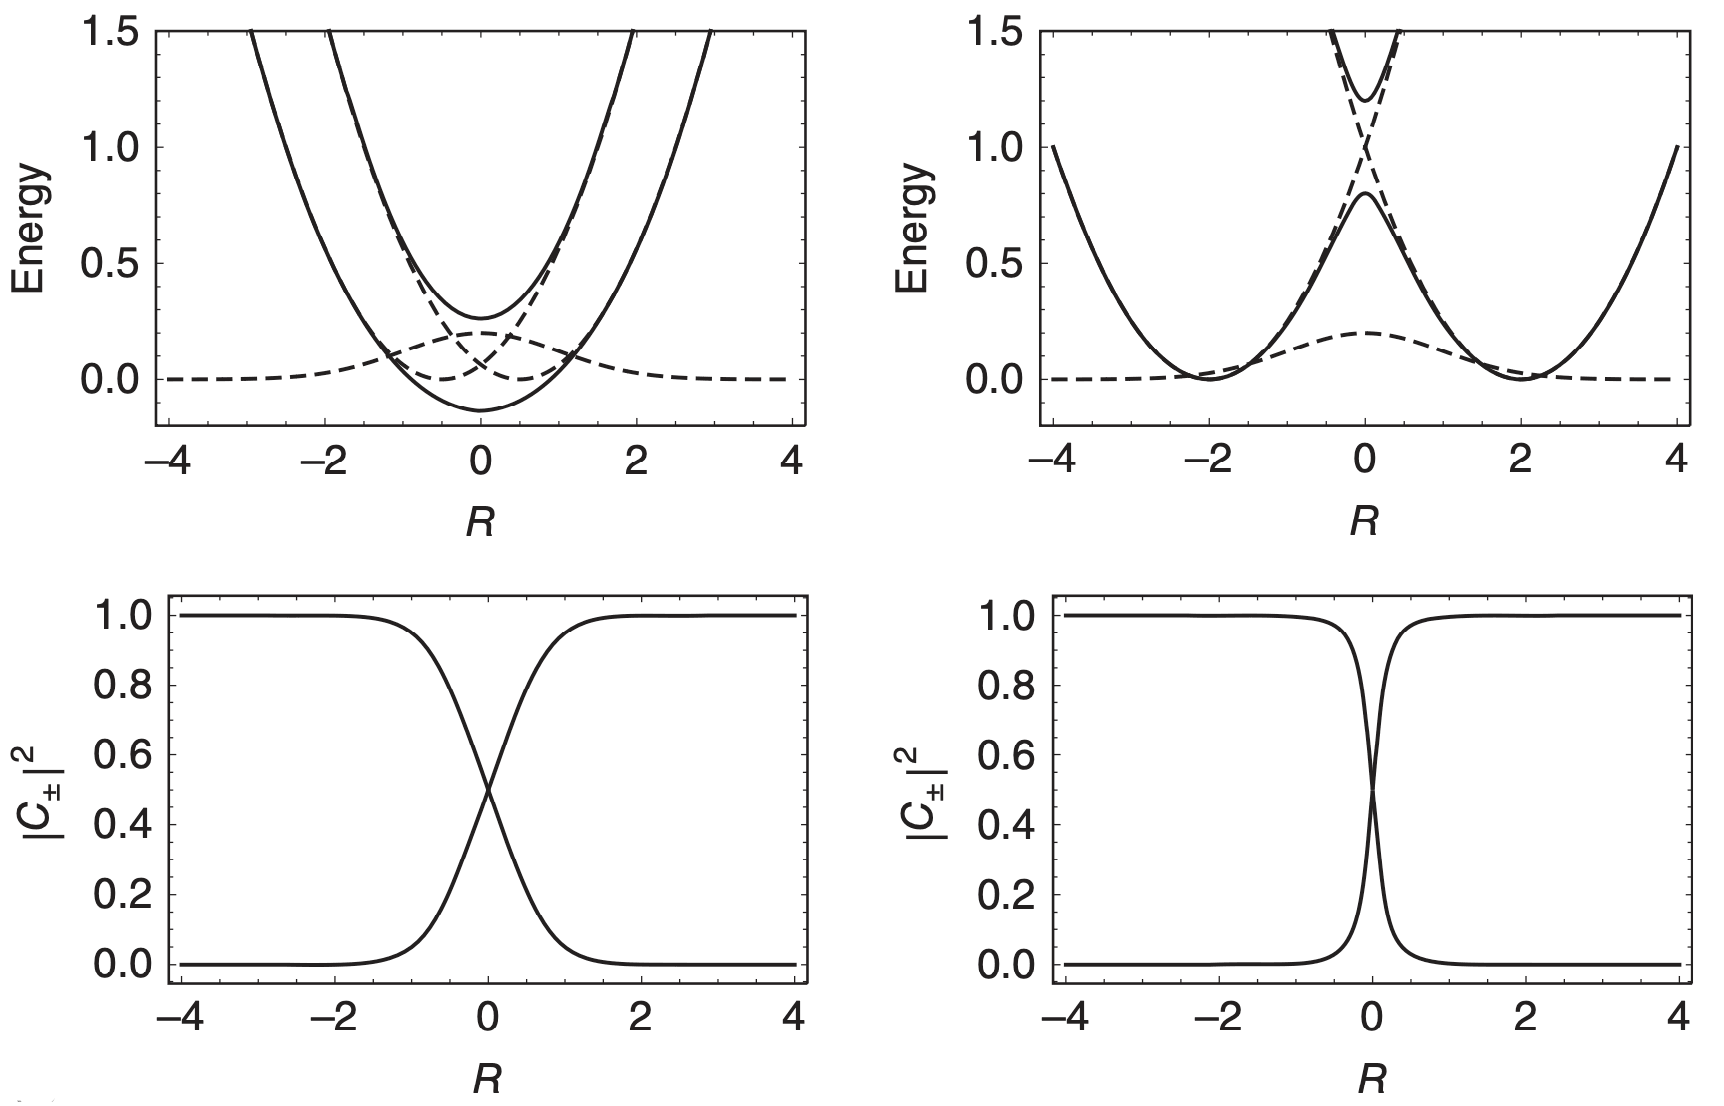
\includegraphics[width=0.75\textwidth]{fig/quantum_chemistry/pes_and_coeff.png}
\caption{\label{fig:tls_e_c}两态系统中(a,b)两种不同绝热势能面的形态以及(c,d)对应的绝热态在透热态上的投影系数。}
\end{figure}

当势能面远离交叉点时，绝热态几乎完全对应于某个透热态，此时$\gamma\approx 0$或$\pi/2$，绝热态在透热态上的投影系数接近于$1$或$0$；当势能面接近交叉点时，$\gamma\approx \pi/4$，绝热态在两个透热态上的投影系数都接近于$1/\sqrt{2}$。因此在交叉点附近，绝热态是两个透热态的混合态，这也是为什么在交叉点附近非绝热跃迁会变得重要的原因。

考虑这个两态系统是电荷转移的给体(D)和受体(A)，我们可以重新描述 Marcus 理论的经典模型：\textcolor{blue}{\textbf{在一维反应坐标$R$上用两个力常数为$\kappa$的谐振子势来描述给体与受体的局域透热势能面$V_{\rm D}^{(d)}(R)=E_{\rm D}+\kappa(R-R_{\rm D})^2/2$和$V_{\rm A}^{(d)}(R)=E_{\rm A}+\kappa(R-R_{\rm A})^2/2$，用一个常数来描述它们之间的电子耦合$V^{(d)}$。}}这样势能矩阵就退化为：
\begin{equation}\label{eq:v_matrix}
\mathbf{V}^{(d)}(R)=
\begin{pmatrix}
E_{\rm D}+\kappa(R-R_1)^2/2 & V^{(d)}\\
V^{(d)} & E_{\rm A}+\kappa(R-R_2)^2/2
\end{pmatrix}    
\end{equation}

\begin{figure}[htbp]
\centering
\includegraphics[width=0.4\textwidth]{fig/quantum_chemistry/marcus.png}
\end{figure}

当然在 Marcus 理论中并不需要处理述势能矩阵 [Eq.\eqref{eq:v_matrix}]，而是观察经典图像，定义重组能(reorganization energy) $\lambda$。它衡量核坐标从给体平衡位置$R_{\rm D}$变到受体平衡位置$R_{\rm A}$所对应的势能代价，即垂直激发能：
\[
\lambda=V_{\rm A}^{(d)}(R_{\rm D})-V_{\rm A}^{(d)}(R_{\rm A})
=V_{\rm D}^{(d)}(R_{\rm A})-V_{\rm D}^{(d)}(R_{\rm D})
=\frac{\kappa}{2}(R_{\rm D}-R_{\rm A})^2
\]
再定义两透热势能面的极小值之差$\Delta G^\circ=E_{\rm A}-E_{\rm D}$\textcolor{blue}{\textbf{（零点能不是自由能，这也算一个近似）}}，其描述了电子转移反应的热力学驱动力。电子转移最容易发生在两张透热势能面简并的位置，即交点$R^\ddagger$处：
\[V_{\rm D}^{(d)}(R^\ddagger)=E_{\rm D}+\frac{\kappa}{2}(R^\ddagger-R_{\rm D})^2=E_{\rm A}+\frac{\kappa}{2}(R^\ddagger-R_{\rm A})^2=V_{\rm A}^{(d)}(R^\ddagger) \quad \Rightarrow \quad R^\ddagger-R_{\rm D}=\frac{R_{\rm A}-R_{\rm D}}{2}\left(1+\frac{\Delta G^\circ}{\lambda}\right)\]
于是从给体极小点爬升到交点所需的活化自由能为：
\[\Delta G^\ddagger=V_{\rm D}^{(d)}(R^\ddagger)-V_{\rm D}^{(d)}(R_{\rm D})=\frac{\kappa}{2}(R^\ddagger-R_{\rm D})^2=\frac{(\lambda+\Delta G^\circ)^2}{4\lambda}\]

在透热表象下电子由发生了不同透热面之间的转移，\textcolor{blue}{\textbf{假设$\lambda\gg|V^{(d)}|$，也即弱耦合极限}}，因此可以由微扰[章节\ref{sec:tdpt}]的结论 Fermi Golden Rule [Eq.\eqref{eq:fgr}]，电子转移速率可以写成：
\[k_{\rm ET}=\frac{2\pi}{\hbar}|V^{(d)}|^2\int \dd{R}\,P_{\rm D}(R)\,\delta\!\left(V_{\rm D}^{(d)}(R)-V_{\rm A}^{(d)}(R)\right)\]
\textcolor{blue}{\textbf{假设温度足够高使得可以使用给体透热面上的经典平衡分布}}（Boltzmann distribution）来描述：
\[P_{\rm D}(R)=\sqrt{\frac{\kappa}{2\pi k_{\mathrm{B}}T}}\exp\left[-\frac{V_{\rm D}^{(d)}(R)-E_{\rm D}}{k_{\mathrm{B}}T}\right]=\sqrt{\frac{\kappa}{2\pi k_{\mathrm{B}}T}}\exp\left[-\frac{\kappa(R-R_{\rm D})^2}{2k_{\mathrm{B}}T}\right]\]
由于两张透热面只在$R^\ddagger$处相交，利用$\delta(f(R))=\delta(R-R^\ddagger)/|f'(R^\ddagger)|$，并注意到：
\[\left|\dv{}{R}\left(V_{\rm D}^{(d)}(R)-V_{\rm A}^{(d)}(R)\right)\right|=\kappa|R_{\rm A}-R_{\rm D}| \quad \Rightarrow \quad k_{\rm ET}=\frac{2\pi}{\hbar}|V^{(d)}|^2\frac{P_{\rm D}(R^\ddagger)}{\kappa|R_{\rm A}-R_{\rm D}|}\]
而在交点处：
\[P_{\rm D}(R^\ddagger)=\sqrt{\frac{\kappa}{2\pi k_{\mathrm{B}}T}}\exp\left(-\frac{\Delta G^\ddagger}{k_{\mathrm{B}}T}\right)\]
再代入$\Delta G^\ddagger=(\lambda+\Delta G^\circ)^2/(4\lambda)$和$\lambda=\kappa(R_{\rm A}-R_{\rm D})^2/2$，便得到著名的 Marcus 速率公式：
\begin{equation}
k_{\rm ET}=\frac{|V^{(d)}|^2}{\hbar}\sqrt{\frac{\pi}{\lambda k_{\mathrm{B}}T}}
\exp\left[-\frac{(\lambda+\Delta G^\circ)^2}{4\lambda k_{\mathrm{B}}T}\right]
\end{equation}
Marcus 理论本质上是“\textcolor{blue}{\textbf{透热双态模型 + 单反应坐标近似 + 抛物线近似 + 高温弱耦合极限}}”的电子转移理论。可以说近似的力度非常之大，但它也能定性或者定量的描述一些性质，其中最著名的就是速率与反应热力学驱动力$\Delta G^\circ$之间的关系：速率并不会随着反应放热程度增大而单调上升。当$\Delta G^\circ$逐渐减小时，速率先增大，并在$\Delta G^\circ=-\lambda$时达到最大，此时$\Delta G^\ddagger=0$，称为无活化电子转移；若继续进入$\Delta G^\circ<-\lambda$的区域，速率反而下降，这个区域就称为 Marcus 反转区。

如果我们不是把电子转移看成发生在两张透热面之间的非绝热跃迁，而是先把上面的势能矩阵 [Eq.\eqref{eq:v_matrix}] 对角化，研究 Marcus 模型的绝热极限。此时决定反应的绝热势能面下支$E_-(R)$为：
\[
E_{-}(R)=\frac{V_{\rm D}^{(d)}(R)+V_{\rm A}^{(d)}(R)}{2}-\frac{1}{2}\sqrt{\left(V_{\rm D}^{(d)}(R)-V_{\rm A}^{(d)}(R)\right)^2+4|V^{(d)}|^2}
\]
此时电子转移就不再是 FGR [Eq.\eqref{eq:fgr}] 意义下的“跃迁”，而更像是沿低绝热面发生的经典越垒过程。如果保留除了透热态意外事件的所有近似，那么我们可以认为：\textcolor{blue}{\textbf{耦合还没有大到把势垒完全抹平，势垒顶仍然靠近前面透热面的交点$R^\ddagger$，而反应物极小点也仍然靠近$R_{\rm D}$}}，则绝热面上的活化自由能$\Delta G_{\rm ad}^{\ddagger}$可以近似为：
\[\Delta G_{\rm ad}^{\ddagger}=E_-(R^{\ddagger})-E_-(R_{\rm D})\approx \Delta G^\ddagger-|V^{(d)}|-\frac{\lambda+\Delta G^\circ}{2}
+\frac{1}{2}\sqrt{(\lambda+\Delta G^\circ)^2+4|V^{(d)}|^2}\]
其中：
\[\begin{aligned}
E_-(R^\ddagger)
&=\frac{V_{\rm D}^{(d)}(R^\ddagger)+V_{\rm A}^{(d)}(R^\ddagger)}{2}
-\frac{1}{2}\sqrt{\left(V_{\rm D}^{(d)}(R^\ddagger)-V_{\rm A}^{(d)}(R^\ddagger)\right)^2+4|V^{(d)}|^2}\\
&=V_{\rm D}^{(d)}(R^\ddagger)-|V^{(d)}|=E_{\rm D}+\Delta G^\ddagger-|V^{(d)}|\\
E_-(R_{\rm D})
&=\frac{V_{\rm D}^{(d)}(R_{\rm D})+V_{\rm A}^{(d)}(R_{\rm D})}{2}-\frac{1}{2}\sqrt{\left(V_{\rm D}^{(d)}(R_{\rm D})-V_{\rm A}^{(d)}(R_{\rm D})\right)^2+4|V^{(d)}|^2}\\
&=E_{\rm D}+\frac{\lambda+\Delta G^\circ}{2}-\frac{1}{2}\sqrt{(\lambda+\Delta G^\circ)^2+4|V^{(d)}|^2}
\end{aligned}\]
需要注意的是，如果要严格求解绝热势能面的能垒$\Delta G_{\rm ad}^{\ddagger}=E_-(R_-^{\ddagger})-E_-(R_-^{\rm min})$需要求解势能面的极小点和势垒顶的位置，应该由$\dd{E_-(R)}/\dd{R}=0$来求解，而不是直接用透热势能面的极小点和交点来近似。在弱耦合极限下，$|V^{(d)}|\ll\lambda<\lambda+\Delta G^\circ$的情况下，上式进一步简化为$\Delta G_{\rm ad}^{\ddagger}\approx \Delta G^\ddagger-|V^{(d)}|$。现在的问题就简化一维（$Q_{\mathrm{DS}}=1$）的经典越垒过程。在高温经典极限下，可以用过渡态理论 [章节\ref{sec:tst}] 来求电子转移速率：
\[k_{\rm ET}^{\rm ad}=\frac{kT}{h} \frac{1}{Q_{\mathrm{R}}} \exp\left(-\frac{\Delta G_{\rm ad}^{\ddagger}}{kT}\right)\]
其中反应物的配分函数$Q_{\mathrm{R}}$由于 Marcus 近似条件可以通过一维谐振子的哈密顿量来求解，由于反应物与过渡态之间的零点能已经被吸收到反应能垒$\Delta G_{\rm ad}^{\ddagger}$中，因此这里的谐振子哈密顿中不需要包含零点能：
\[Q_{\mathrm{R}}=\int\frac{\dd{R}\dd{P}}{2\pi\hbar}\exp\left[-\beta H_-(R,P)\right]\approx\int\frac{\dd{R}\dd{P}}{2\pi\hbar}\exp\left[-\beta\left(\frac{P^2}{2M}+\frac{1}{2}M\omega_{\rm r}^2(R-R_-^{\rm min})^2\right)\right]=\frac{1}{\beta\hbar\omega_{\rm r}}\]
这里$M$是反应坐标的有效质量，$\omega_{\rm r}$是反应物谷中核坐标的振动频率，满足$\kappa=M\omega_{\rm r}^2$。因此电子转移速率为：
\begin{equation}
k_{\rm ET}^{\rm ad}=\frac{kT}{h} \beta\hbar\omega_{\rm r} \exp\left(-\frac{\Delta G_{\rm ad}^{\ddagger}}{kT}\right)\approx\frac{\omega_{\rm r}}{2\pi}\exp\left(-\frac{\Delta G^\ddagger-|V^{(d)}|}{kT}\right)=\frac{\omega_{\rm r}}{2\pi}\exp\left[\frac{|V^{(d)}|}{kT}-\frac{(\lambda+\Delta G^\circ)^2}{4\lambda k_{\mathrm{B}}T}\right]
\end{equation}

这就是绝热极限下的 Marcus 速率公式。电子耦合$V^{(d)}$的作用主要体现在改变了绝热能垒$\Delta G_{\rm ad}^{\ddagger}$。这说明在绝热极限下，电子耦合增强时速率上升主要不是因为“跃迁概率”变大，而是因为 avoided crossing 附近的低绝热面被压低，从而减小了越垒所需的活化能。从下图可以发现当给体和受体的透热势能面对称时，非绝热耦合$V^{(d)}$的增加会使得绝热能垒$\Delta G_{\rm ad}^{\ddagger}$迅速降低，因此速率会迅速增加；当给体和受体的透热势能面不对称时，非绝热耦合$V^{(d)}$的增加对绝热能垒$\Delta G_{\rm ad}^{\ddagger}$的影响就没有那么大，因此速率的增加也没有那么大。这也说明了为什么在 Marcus 反转区中，非绝热耦合增强时速率的提升并不明显。

\begin{figure}[htbp]
\centering
\includegraphics[width=0.5\textwidth]{fig/quantum_chemistry/marcus_pes.png}
\end{figure}

\newpage
\section{Slater-Condon 规则}
在BO近似后，电子哈密顿如下：
\[\hat{H}_{\rm el}=\hat{T}_{\rm el}+\hat{V}_{\rm nuc-nuc}+\hat{V}_{\rm nuc-el}+\hat{V}_{\rm el-el}=-\sum_{i=1}^N\frac{1}{2}\nabla^2_{\mathbf{r},i}+\sum_{I=1}^{M}\sum_{J>I}^{M}\frac{Z_{I}Z_{J}}{|\mathbf{R}_{I}-\mathbf{R}_{J}|}-\sum_{i=1}^{N}\sum_{I=1}^{M}\frac{Z_{I}}{|\mathbf{r}_{i}-\mathbf{R}_{I}|}+\sum_{i=1}^{N}\sum_{j>i}^{N}\frac{1}{|\mathbf{r}_{i}-\mathbf{r}_{j}|}\]

虽然我们已经把核动能项给舍去了，但电子部分的哈密顿依然包含二体的电子之间的库伦相互作用，还是一个难以处理的部分。我们一般好处理的都是单体问题，比如氢原子的电子薛定谔（固定原子核）、谐振子等等，所以我们希望能将多体问题尽可能精确地转换为单体问题来处理，如我们之前提到的平均场近似，如此一来多电子问题就被转换为了单电子问题。相对应的，体系的波函数也变成了几个单体波函数(自旋轨道)的乘积（Hartree 基）$\ket{\Psi}=\ket{\phi_1}\otimes\ket{\phi_2}\otimes\cdots\otimes\ket{\phi_n}:=\ket{\phi_1\phi_2\cdots\phi_n}$。但由于电子费米子的全同性的要求，上述需要对 Hartree 基做反对称化得到 Slater 行列式$\ket{\Psi}=\hat{A}(\ket{\phi_1}\otimes\ket{\phi_2}\otimes\cdots\otimes\ket{\phi_n}):=\hat{A}\ket{\phi_1\phi_2\cdots\phi_n}$。

在此基础上，我们希望能计算出 Slater 行列式$\ket{\Psi}$对哈密顿量$\hat{H}$的期望值$\bra{\Psi}\hat{H}\ket{\Psi}$，但直接计算会非常复杂，为此我们引入 Slater-Condon 规则来简化计算。
\begin{theorem}[Slater-Condon 规则]\label{slater-condon}
设$\ket{\Psi}$和$\ket{\Psi'}$为由正交归一的自旋轨道组成的 Slater 行列式，则其对单体算符$\hat{F}$和双体算符$\hat{G}$
\[\hat{F}=\sum_i\hat{f}_i, \quad \hat{G}=\sum_{i<j}\hat{g}_{ij}\]
的矩阵元分别为：
\begin{itemize}
\item 若$\ket{\Psi'}=\ket{\Psi}$，则：
\[\bra{\Psi}\hat{F}\ket{\Psi}=\sum_i\bra{i}\hat{f}_i\ket{i}, \quad \bra{\Psi}\hat{G}\ket{\Psi}=\frac{1}{2}\sum_{i,j}(\bra{ij}\hat{g}_{ij}\ket{ij}-\bra{ij}\hat{g}_{ij}\ket{ji})\]
其中：
\[\bra{ij}\ket{kl}=\iint \psi_i^*(\bm{r}_1)\psi_j^*(\bm{r}_2)\hat{g}(1,2)\psi_k(\bm{r}_1)\psi_l(\bm{r}_2)\dd{\bm{r}_1}\dd{\bm{r}_2}\]
\item 若$\ket{\Psi'}$与$\ket{\Psi}$仅有一个自旋轨道不同，设$\ket{\Psi'}=\hat{a}_r^{\dagger}\hat{a}_s\ket{\Psi}$，则：
\[\bra{\Psi'}\hat{F}\ket{\Psi}=\bra{r}\hat{f}_r\ket{s}, \quad \bra{\Psi'}\hat{G}\ket{\Psi}=\sum_{i}(\bra{ri}\hat{g}_{ri}\ket{si}-\bra{ri}\hat{g}_{ri}\ket{is})\]
\item 若$\ket{\Psi'}$与$\ket{\Psi}$有两个自旋轨道不同，设$\ket{\Psi'}=\hat{a}_r^{\dagger}\hat{a}_s^{\dagger}\hat{a}_u\hat{a}_v\ket{\Psi}$，则：
\[\bra{\Psi'}\hat{F}\ket{\Psi}=0, \quad \bra{\Psi'}\hat{G}\ket{\Psi}=\bra{rs}\hat{g}_{rs}\ket{uv}-\bra{rs}\hat{g}_{rs}\ket{vu}\]
\item 若$\ket{\Psi'}$与$\ket{\Psi}$有超过两个自旋轨道不同，则：
\[\bra{\Psi'}\hat{F}\ket{\Psi}=0, \quad \bra{\Psi'}\hat{G}\ket{\Psi}=0\]
\end{itemize}
\end{theorem}
\begin{proof}
考虑以正交归一的一组自旋轨道构建的 Slater 行列式$\ket{\Psi}=\hat{A}\ket{\phi_1\phi_2\cdots\phi_n}$，反对称化算符显然有一下性质$\hat{A}=\hat{A}^{\dagger}, \ \hat{A}^2=\sqrt{n!}\hat{A}$（把任意一个位置调换算符作用到反对称化的波函数上只能获得其自身）。因此对overlap：
\[\bra{\Psi}\ket{\Psi}=\bra{\phi_1\phi_2\cdots\phi_n}\sum_k\epsilon_k\hat{P}_k\ket{\phi_1\phi_2\cdots\phi_n}=\bra{\phi_1\phi_2\cdots\phi_n}\ket{\phi_1\phi_2\cdots\phi_n}=1\]
只有完全没被调换过粒子编号的态才有不为0的内积，如果不是相同态的内积$\bra{\Psi'}\ket{\Psi}$显然为0，因为根本不可能通过对调获得完全一样的态。

类似的对于单体算符$\hat{f}_i$，这里角标$i$表示自旋轨道，用相同的态做内积，只有没被调换过的态有非0结果：
\[\bra{\Psi}\hat{f}_i\ket{\Psi}=\bra{\phi_1\phi_2\cdots\phi_n}\sum_k\epsilon_k\hat{f}_i\hat{P}_k\ket{\phi_1\phi_2\cdots\phi_n}=\bra{\phi_1\phi_2\cdots\phi_n}\hat{f}_i\ket{\phi_1\phi_2\cdots\phi_n}=\bra{\phi_i}\hat{f}_i\ket{\phi_i}\]
这里需要注意轨道角标表示自旋轨道的编号，而算符$\hat{P}_k$是作用到电子编号上的，其角标$k$表示一种对调方式。

如果是不同的态作用到单体算符上，则至多只能有一个轨道不一样且该不同的轨道必须包含在单体算符的期望值项里（假设$\ket{\Psi'}=\hat{a}_r^{\dagger}\hat{a}_s\ket{\Psi}$）：
\[\bra{\Psi'}\hat{f}_r\ket{\Psi}=\bra{\phi_r\phi_2\cdots\phi_n}\sum_k\epsilon_k\hat{f}_r\hat{P}_k\ket{\phi_s\phi_2\cdots\phi_n}=\bra{\phi_r\phi_2\cdots\phi_n}\hat{f}_r\ket{\phi_s\phi_2\cdots\phi_n}=\bra{\phi_r}\hat{f}_r\ket{\phi_s}\]
最后带入单体算符$\hat{F}$的定义我们可以得到：
\[\bra{\Psi}\hat{F}\ket{\Psi}=\bra{\Psi}\sum_{i=1}^{n}\hat{f}_i\ket{\Psi}=\sum_{i=1}^{n}\bra{\phi_i}\hat{f}_i\ket{\phi_i}, \quad \bra{\Psi'}\hat{F}\ket{\Psi}=\bra{\phi_r\phi_2\cdots\phi_n}\sum_{i=1}^{n}\hat{f}_i\ket{\phi_s\phi_2\cdots\phi_n}=\bra{\phi_r}\hat{f}_r\ket{\phi_s}\]

对于一个态，对掉一次至少两个轨道不一样，对掉两次（注意不包含换回来）则不一样的更多，对单体算符由于只允许一个轨道不一样所以不可能允许存在对掉一次的组分，对双体算符也只允许对掉一次，因此对于双体算符$\hat{g}_{ij}$的期望值可以很轻易得写出：
\[\bra{\Psi}\hat{G}\ket{\Psi}=\bra{\Psi}\sum_{i<j}\hat{g}_{ij}\ket{\Psi}=\sum_{i<j}\bra{\phi_i\phi_j}\hat{g}_{ij}(1-\hat{P}_{12})\ket{\phi_i\phi_j}=\frac{1}{2}\sum_{i,j}\bra{\phi_i\phi_j}\hat{g}_{ij}(1-\hat{P}_{12})\ket{\phi_i\phi_j}\]
对单替换行列式$\ket{\Psi'}=\hat{a}_r^{\dagger}\hat{a}_s\ket{\Psi}$，只有当$\hat{g}_{ij}$作用在包含了不同轨道的那一对轨道上时才有非0结果：
\[\bra{\Psi'}\hat{G}\ket{\Psi}=\sum_{i}\bra{\phi_r\phi_i}\hat{g}_{ri}(1-\hat{P}_{12})\ket{\phi_s\phi_i}\]
对双替换行列式$\ket{\Psi''}=\hat{a}_r^{\dagger}\hat{a}_s^{\dagger}\hat{a}_u\hat{a}_v\ket{\Psi}$，只有当$\hat{g}_{ij}$作用在包含了不同轨道的那一对轨道上时才有非0结果：
\[\bra{\Psi''}\hat{G}\ket{\Psi}=\bra{\phi_r\phi_s}\hat{g}_{rs}(1-\hat{P}_{12})\ket{\phi_u\phi_v}\]
更高阶的替换将会在除了作用在算符上的轨道之外的 overlap 部分出现无法匹配的情况，因此结果为0。
\end{proof}

\section{Hartree-Fock}
\subsection{Hartree近似与 Hartree 有效势}\label{sec:hartree}
在 BO 近似之后，虽然核动能项已经被舍去，但电子哈密顿量里依然包含电子-电子之间的双体库伦相互作用，因此多电子薛定谔方程仍然无法精确求解。最直接的想法就是先把这个多电子问题尽可能地改写成单电子问题。最朴素的近似是暂时忽略双体项，只保留单电子哈密顿量（Hartree 近似）：
\[\hat{H}\approx\sum_i\hat{h}_i=-\sum_{i=1}^N\frac{1}{2}\nabla^2_{\mathbf{r},i}-\sum_{i=1}^{N}\sum_{I=1}^{M}\frac{Z_{I}}{|\mathbf{r}_{i}-\mathbf{R}_{I}|}\]
此时体系波函数自然可以近似写成若干单电子轨道的直积$\Psi^{\rm H}(\bm{r}_1,\bm{r}_2,\cdots,\bm{r}_N)=\psi_1(\bm{r}_1)\psi_2(\bm{r}_2)\cdots\psi_N(\bm{r}_N)$，这样的多电子波函数也被称为 Hartree 积，且每个轨道都满足独立的单电子方程：
\[\hat{h}\psi_i(\bm{r})=\varepsilon_i\psi_i(\bm{r}), \quad E\approx\sum_i\varepsilon_i\]
Hartree 近似把体系完全当成互不相互作用的独立电子来处理，体系能量$E$可以近似为轨道能量$\varepsilon_i$之和，但是该近似显然过于粗糙。更进一步地，我们不直接把电子-电子相互作用整个丢掉，而是把它近似成每个电子感受到的其他电子产生的平均静电势，也就是 Hartree 有效势，这一思想也即平均场（Mean field）近似的来源：
\[\left[\hat{h}+V_i^{\rm H}(\bm{r})\right]\psi_i(\bm{r})=\varepsilon_i\psi_i(\bm{r}), \quad V_i^{\rm H}(\bm{r})=\sum_{j\ne i}\int\frac{|\psi_j(\bm{r}')|^2}{|\bm{r}-\bm{r}'|}\dd{\bm{r}'}\]
由于每个轨道感受到不同的有效势，同时这些轨道要满足正交归一的限制条件，因此上述 Hartree 方程的求解在数学上并不简单。通常所说的 Hartree 近似是指如下更为简单的方程：
\[\left[\hat{h}+V_{\rm eff}^{\rm H}(\bm{r})\right]\psi_i(\bm{r})=\left[\hat{h}+\int\frac{\rho(\bm{r}')}{|\bm{r}-\bm{r}'|}\dd{\bm{r}'}\right]\psi_i(\bm{r})=\varepsilon_i\psi_i(\bm{r}), \quad \rho(\bm{r})=\sum_j|\psi_j(\bm{r})|^2\]
由于$V_{\rm eff}^{\rm H}$本身依赖于所有轨道，这组方程不能一次直接解出，而必须通过不断更新轨道和势能直到收敛，这已经是 SCF 思想的雏形。不过 Hartree 方法虽然引入了平均场库伦势，但它仍然使用 Hartree 乘积作为波函数，不满足电子作为费米子的反对称性要求，也不会自动包含交换作用。沿着“平均场”这条思路再向前迈一步，把试探波函数从 Hartree 乘积升级为 Slater 行列式，就得到了 Hartree-Fock 方法。

\subsection{正则轨道下的 Hartree-Fock}\label{sec:hf}
前一小节中我们先看到了两个最直接的单电子化近似：完全忽略双体项的 Hartree 近似，以及把电子-电子相互作用替换成平均库伦势的 Hartree 方法。它们都保留了“每个电子在某个有效单电子势中运动”的 Mean field 思想，但 Hartree 乘积不满足费米子的反对称性要求，也无法自然给出交换效应。Hartree-Fock 方法正是在这里向前迈出的关键一步：它仍然利用变分法把精确哈密顿量近似成单电子算符的和，但试探波函数不再取 Hartree 乘积，而是改用由正交归一自旋轨道构成的 Slater 行列式。这样一来，交换项会在变分过程中自动出现。从 HF 出发，如果我们认为\textcolor{red}{\textbf{ Slater 行列式形式的波函数}}已经足够好而\textcolor{blue}{\textbf{近似的单电子哈密顿量}}还不够精确，就会得到 MP 等微扰方法；反过来，如果我们认为\textcolor{blue}{\textbf{近似的单电子哈密顿量}}是精确的而\textcolor{red}{\textbf{ Slater 行列式形式的波函数}}还不够好，那么从 Slater 行列式出发就会走向 CI, CC, MCSCF 等方法。

由Condon-Slater规则 [定理\ref{slater-condon}]，正则轨道(正交归一的自旋轨道)组成的 Slater 行列式$\ket{\Psi}$对哈密顿量$\hat{H}$的期望（能量$E$）如下所示，其中$\bra{ij}\ket{ij},\bra{ij}\ket{ji}$为库伦积分和交换积分，$h_i$包括了动能项和核对电子的势能：
\[E=\bra{\Psi}\hat{H}\ket{\Psi}=\sum_ih_i+\frac{1}{2}\sum_{i,j}\left(\bra{ij}\ket{ij}-\bra{ij}\ket{ji}\right)\]
通过拉格朗日乘数法把正交归一条件引入泛函$\eta[\{\psi_i\},\lambda_{ij}]$进行变分，这里变分的目的是寻找到最佳的一组单电子轨道波函数$\{\psi_i\}$使得能量最小化，通过变分我们会获得一组单电子波函数$\{\psi_i\}$的约束方程。约定符号$\bra{\bm{r}}\ket{i}=\psi_i(\bm{r})\equiv\psi_i$，采用波函数表象时定义变分泛函为：
\begin{equation*}
\begin{aligned}
\eta[\{\psi_i\},\lambda_{ij}]&=\sum_i\int \psi_i^*(\bm{r})\hat{h}\psi_i(\bm{r})\dd{\bm{r}}\\
&\quad+\frac{1}{2}\sum_{i,j}\iint\frac{\psi_i^*(\bm{r}_1)\psi_j^*(\bm{r}_2)\psi_i(\bm{r}_1)\psi_j(\bm{r}_2)-\psi_i^*(\bm{r}_1)\psi_j^*(\bm{r}_2)\psi_j(\bm{r}_1)\psi_i(\bm{r}_2)}{r_{12}}\dd{\bm{r}_1}\dd{\bm{r}_2}\\
&\quad-\sum_{i,j}\lambda_{ij}\left(\int \psi_i^*(\bm{r})\psi_j(\bm{r})\dd{\bm{r}}-\delta_{ij}\right)
\end{aligned}
\end{equation*}

对$\psi_p^*$做泛函变分，这里$p$表示被变分的轨道指标，以避免与泛函中求和指标$i,j$混淆。单电子项直接给出：
\[\frac{\delta}{\delta \psi_p^*}\sum_i\int \psi_i^*(\bm{r}')\hat{h}\psi_i(\bm{r}')\dd{\bm{r}'}=\hat{h}\psi_p(\bm{r})\]
对双电子中的库伦项，有：
\[\begin{aligned}
\frac{1}{2}\frac{\delta}{\delta \psi_p^*}
&\sum_{i,j}\iint
\frac{\psi_i^*(\bm{r}_1)\psi_j^*(\bm{r}_2)\psi_i(\bm{r}_1)\psi_j(\bm{r}_2)}{r_{12}}
\dd{\bm{r}_1}\dd{\bm{r}_2}\\
&=\frac{1}{2}\sum_j\left(\int\frac{|\psi_j(\bm{r}')|^2}{|\bm{r}-\bm{r}'|}\dd{\bm{r}'}\right)\psi_p(\bm{r})+\frac{1}{2}\sum_i\left(\int\frac{|\psi_i(\bm{r}')|^2}{|\bm{r}-\bm{r}'|}\dd{\bm{r}'}\right)\psi_p(\bm{r})\\
&=\sum_j\left(\int\frac{|\psi_j(\bm{r}')|^2}{|\bm{r}-\bm{r}'|}\dd{\bm{r}'}\right)\psi_p(\bm{r})\equiv\sum_j\hat{J}_j\psi_p(\bm{r})
\end{aligned}\]
同理，交换项的变分为：
\[\begin{aligned}
-\frac{1}{2}\frac{\delta}{\delta \psi_p^*}
&\sum_{i,j}\iint
\frac{\psi_i^*(\bm{r}_1)\psi_j^*(\bm{r}_2)\psi_j(\bm{r}_1)\psi_i(\bm{r}_2)}{r_{12}}
\dd{\bm{r}_1}\dd{\bm{r}_2}\\
&=-\frac{1}{2}\sum_j\left(\int\frac{\psi_j^*(\bm{r}')\psi_p(\bm{r}')}{|\bm{r}-\bm{r}'|}\dd{\bm{r}'}\right)\psi_j(\bm{r})-\frac{1}{2}\sum_i\left(\int\frac{\psi_i^*(\bm{r}')\psi_p(\bm{r}')}{|\bm{r}-\bm{r}'|}\dd{\bm{r}'}\right)\psi_i(\bm{r})\\
&=-\sum_j\left(\int\frac{\psi_j^*(\bm{r}')\psi_p(\bm{r}')}{|\bm{r}-\bm{r}'|}\dd{\bm{r}'}\right)\psi_j(\bm{r})\equiv-\sum_j\hat{K}_j\psi_p(\bm{r})
\end{aligned}\]
而正交归一约束项给出：
\[-\frac{\delta}{\delta \psi_p^*}\sum_{i,j}\lambda_{ij}\left(\int \psi_i^*(\bm{r}')\psi_j(\bm{r}')\dd{\bm{r}'}-\delta_{ij}\right)=-\sum_j\lambda_{pj}\psi_j(\bm{r})\]
将被变分的轨道指标$p$重新记回常用的$i$，得到单电子轨道的约束方程：
\[\hat{F}\psi_i(\bm{r})=\left[\hat{h}+\sum_j(\hat{J}_j-\hat{K}_j)\right]\psi_i(\bm{r})=\sum_j\lambda_{ij}\psi_j(\bm{r}), \quad \hat{F}=\hat{h}+\sum_j(\hat{J}_j-\hat{K}_j)\]
其中$\hat{F},\hat{h},\hat{J}_j,\hat{K}_j$分别为 Fock 算符，单电子算符，库伦算符和交换算符。

对上式左乘$\psi_k^*(\bm{r})$并积分：
\[\int \psi_k^*(\bm{r})\hat{F}\psi_i(\bm{r})\dd{\bm{r}}=\sum_j\lambda_{ij}\int \psi_k^*(\bm{r})\psi_j(\bm{r})\dd{\bm{r}}=\sum_j\lambda_{ij}\delta_{kj}=\lambda_{ik}\]
另一方面，由于$\hat{h},\hat{J}_j,\hat{K}_j$都是厄密算符，故$\hat{F}$也是厄密算符，因此：
\[\lambda_{ik}=\int \psi_k^*(\bm{r})\hat{F}\psi_i(\bm{r})\dd{\bm{r}}=\left(\int \psi_i^*(\bm{r})\hat{F}\psi_k(\bm{r})\dd{\bm{r}}\right)^*=\lambda_{ki}^*\]
因此$\lambda_{ij}$构成厄密矩阵。由于占据轨道之间的酉变换不改变 Slater 行列式表示的能量，因此总可以在占据子空间内再做一次酉变换将其对角化，得到每个轨道对应的轨道能量$\varepsilon_i$，于是得到正则轨道下的 Hartree-Fock 方程和对应的平均场哈密顿量$\hat{H}_0$：
\[\hat{F}\psi_i(\bm{r})=\varepsilon_i\psi_i(\bm{r}), \quad \hat{H}_0=\sum_i\hat{F}_i=\sum_i\left(\hat{h}(i)+\sum_j(\hat{J}_j-\hat{K}_j)\right)\]
其中轨道能量$\varepsilon_i$就是对角化后的拉格朗日乘子。库伦算符$\hat{J}_i$和交换算符$\hat{K}_i$的定义如下：
\[\hat{J}_j\psi_i(\bm{r})=\left(\int\frac{|\psi_j(\bm{r}')|^2}{|\bm{r}-\bm{r}'|}\dd{\bm{r}'}\right)\psi_i(\bm{r}), \quad \hat{K}_j\psi_i(\bm{r})=\left(\int\frac{\psi_j^*(\bm{r}')\psi_i(\bm{r}')}{|\bm{r}-\bm{r}'|}\dd{\bm{r}'}\right)\psi_j(\bm{r})\]
将双电子平均场部分打包成$\hat{G}=\sum_j(\hat{J}_j-\hat{K}_j)$，则其期望值为：
\[\begin{aligned}
\int \psi_i^*(\bm{r})\hat{G}\psi_i(\bm{r})\dd{\bm{r}}&=\sum_j\iint\frac{\psi_i^*(\bm{r}_1)\psi_j^*(\bm{r}_2)\psi_i(\bm{r}_1)\psi_j(\bm{r}_2)-\psi_i^*(\bm{r}_1)\psi_j^*(\bm{r}_2)\psi_j(\bm{r}_1)\psi_i(\bm{r}_2)}{r_{12}}\dd{\bm{r}_1}\dd{\bm{r}_2}\\
&=\sum_{j}(\bra{ij}\ket{ij}-\bra{ij}\ket{ji})
\end{aligned}\]

通过变分法我们直接得到的首先只是“最优轨道必须满足什么方程”，也就是自洽轨道约束方程（Hartree-Fock 方程），这个轨道方程告诉我们：在 Slater 行列式这个受限变分空间中，\textcolor{blue}{\textbf{每个电子都等效地在同一个由其他电子平均作用产生的单电子 Fock 算符$\hat{F}$下运动}}。我们把相应的多电子平均场问题定义为这些单电子算符之和$\hat{H}_0=\sum_i\hat{F}_i$。换句话说，\textcolor{blue}{\textbf{$\hat{H}_0$不是由$\hat{H}$严格推出的全空间算符恒等变换，而是在 Slater 行列式近似下与变分极值条件等价的最优单电子平均场哈密顿量}}。

如果我们考虑空间轨道，则 HF 可以分为 RHF (闭壳层，电子成对)，UHF (开壳层，不同自旋单独考虑)和 ROHF (开壳层，部分成对部分单独)。对 UHF 之需要简单写两套能量加起来就好：
\[E_{\rm{UHF}}=\sum_{i,\uparrow}h_i+\frac{1}{2}\sum_{i,j,\uparrow}\left(\bra{ij}\ket{ij}-\bra{ij}\ket{ji}\right)+\sum_{i,\downarrow}h_i+\frac{1}{2}\sum_{i,j,\downarrow}\left(\bra{ij}\ket{ij}-\bra{ij}\ket{ji}\right)\]
ROHF 太复杂先不说，看看 RHF 能量：
\[E_{\rm{RHF}}=2\sum_ih_i+\sum_{i,j}\left(2\bra{ij}\ket{ij}-\bra{ij}\ket{ji}\right)\]
对单电子项，只有自己会跟自己的作用，所以写成空间轨道后加倍，库伦积分也类似，轨道只跟自己积分，但由于涉及了两个轨道，所以翻四倍，而交换积分涉及不同轨道积分，只有自旋相同的积分不为零，因此加倍。

可以看到在 HF 中不同自旋的电子没有相互作用，可以同时出现在一个轨道上，但实际上由于瞬时库伦相互作用，电子会排斥其他电子出现在其附近(Coulomb hole)，这部分相互作用我们称之为\textcolor{blue}{\textbf{动态相关}}。另外的，当体系中存在近简并态时，单 Slater 行列式无法描述电子在这些近简并态间的跃迁（即存在多个不同的电子组态对体系影响重大，每一个电子组态对应一个 Slater 行列式，因此需要多个 Slater 行列式才能描述清楚系统的电子结构），这部分相互作用我们称之为\textcolor{blue}{\textbf{静态相关}}。HF 方法由于忽略了电子相关，因此计算结果一般会高于真实能量。

\subsection{Hartree-Fock-Roothaan 方法}
假定正则轨道被已知的原子轨道基底下展开，则在此基底下 Fock 矩阵和 overlap 矩阵为：
\[\ket{\psi_i}=\sum_{\nu}c_{\nu i}\ket{\phi_{\nu}} \quad \Leftrightarrow \quad \bm{\Psi}=\bm{\Phi}\mathbf{C}, \quad F_{\mu\nu}=\bra{\phi_{\mu}}\hat{F}\ket{\phi_{\nu}}, \quad S_{\mu\nu}=\bra{\phi_{{\mu}}}\ket{\phi_{\nu}}\]
将基函数带入Hartree-Fock方程后写成矩阵形式(Hartree-Fock-Roothaan 方程)：
\[\bra{\phi_{\mu}}\hat{F}\ket{\psi_i}=\varepsilon_i\bra{\phi_{\mu}}\ket{\psi_i} \quad \Rightarrow \quad \sum_{\nu}c_{\nu i}\bra{\phi_{\mu}}\hat{F}\ket{\phi_{\nu}}=\varepsilon_i\sum_{\nu}c_{\nu i}\bra{\phi_{\mu}}\ket{\phi_{\nu}} \quad \Leftrightarrow \quad \mathbf{F}\mathbf{C}=\mathbf{S}\mathbf{C}\bm{\varepsilon}\]
以上方程的对角化与一般厄密矩阵(这里是实对称阵)的正交对角化$\mathbf{F}\mathbf{C}'=\mathbf{C}'\varepsilon$不一样，考虑 overlap 的酉变换：
\[\mathbf{X}^{\dagger}\mathbf{S}\mathbf{X}=\mathbf{s} \quad \Rightarrow \quad \mathbf{s}^{-1/2}\mathbf{X}^{\dagger}\mathbf{S}\mathbf{X}\mathbf{s}^{-1/2}=\mathbf{U}^{\dagger}\mathbf{S}\mathbf{U}=\mathbf{1} \quad \Rightarrow \quad \mathbf{U}=\mathbf{X}\mathbf{s}^{-1/2}\]
其中$\mathbf{X}$，$\mathbf{s}$为$\mathbf{S}$正交对角化的变换矩阵和对角阵，$\mathbf{s}^{-1/2}$为对角阵$\mathbf{s}^{-1}$的开方，其定义为$\mathbf{s}^{-1/2}\mathbf{s}^{-1/2}=\mathbf{s}^{-1}$。
通过酉变换$\mathbf{U}$将基底变换到标准正交基，在新的基底下系数$\mathbf{C}'$与原系数$\mathbf{C}$的关系$\mathbf{C}=\mathbf{U}\mathbf{C}'$：
\[\mathbf{F}\mathbf{C}=\mathbf{S}\mathbf{C}\bm{\varepsilon} \quad \Rightarrow \quad \mathbf{F}\mathbf{U}\mathbf{C}'=\mathbf{S}\mathbf{U}\mathbf{C}'\bm{\varepsilon} \quad \Rightarrow \quad \mathbf{U}^{\dagger}\mathbf{F}\mathbf{U}\mathbf{C}'=\mathbf{U}^{\dagger}\mathbf{S}\mathbf{U}\mathbf{C}'\bm{\varepsilon}\quad \Rightarrow \quad \mathbf{F}'\mathbf{C}'=\mathbf{C}'\bm{\varepsilon}\]
经过上述酉变换即可得到可对角化的矩阵方程。实际上在 python 中使用 scipy.linalg.eigh($\mathbf{F}$,$\mathbf{S}$) 就能直接解出$\mathbf{C}$。但求解 Hartree-Fock-Roothaan 方程真的只是做一个对角化吗，如果是这样就好了。我们具体来看每个矩阵的具体形式，系数矩阵和 overlap 矩阵是简单的，fock 矩阵包含了单电子积分和双电子积分：
\[F_{\mu\nu}=\bra{\phi_{\mu}}\hat{F}\ket{\phi_{\nu}}=\bra{\phi_{\mu}}\hat{h}\ket{\phi_{\nu}}+\sum_j\bra{\phi_{\mu}}(\hat{J}_j-\hat{K}_j)\ket{\phi_{\nu}}\]
其中双电子部分：
\begin{equation*}
\begin{aligned}
\sum_j\bra{\phi_{\mu}}(\hat{J}_j-\hat{K}_j)\ket{\phi_{\nu}}&=\sum_{j}(\bra{\phi_{\mu}j}\ket{\phi_{\nu}j}-\bra{\phi_{\mu}j}\ket{j\phi_{\nu}})=\sum_{rs}\sum_{j}c_{rj}^*c_{sj}(\bra{\phi_{\mu}\phi_r}\ket{\phi_{\nu}\phi_s}-\bra{\phi_{\mu}\phi_r}\ket{\phi_s\phi_{\nu}})\\
&=\sum_{rs}P_{rs}(\bra{\phi_{\mu}\phi_r}\ket{\phi_{\nu}\phi_s}-\bra{\phi_{\mu}\phi_r}\ket{\phi_s\phi_{\nu}})=\sum_{rs}P_{rs}\bra{\phi_{\mu}\phi_r}\ket{|\phi_{\nu}\phi_s}\\
\end{aligned}
\end{equation*}
这里我们定义了一个新符号$\bra{\phi_{\mu}\phi_r}\ket{|\phi_{\nu}\phi_s}=\bra{\phi_{\mu}\phi_r}\ket{\phi_{\nu}\phi_s}-\bra{\phi_{\mu}\phi_r}\ket{\phi_s\phi_{\nu}}$简化书写。

上式中$P_{\alpha\beta}$是密度矩阵$\mathbf{P}$的矩阵元，显然我们知道密度矩阵可以由系数矩阵得到$\mathbf{P}=\mathbf{C}\Lambda\mathbf{C}^{\dagger}$，其中$\Lambda$表示每个正则轨道的占据数，与我们对体系的要求有关（见下文），密度矩阵具有以下性质：
\[1. \ \mathbf{P}=\mathbf{P}^{\dagger}, \quad 2. \ \mathbf{P}\mathbf{S}\mathbf{P}=\mathbf{P}, \quad 3.\ \text{Tr}(\mathbf{P}\mathbf{S})=N\]
显然密度矩阵也跟采用 R，U 还是 RO 有关，比如在 pySCF 中，密度矩阵通过 1RDM=coeff*mo\_occ*coeff.T 表示，其中 coeff 是系数矩阵，表示从原子轨道到所有正则轨道的变换（基数量守恒，无关是非填入电子），mo\_occ表示轨道占据数。对 R，占据情况只有0和2，对 RO，有0，1和2，对 U 则是两套独立的0和1。

所以事实上\textcolor{blue}{\textbf{需要对角化的 Fock 矩阵也是需要系数矩阵来计算的，因而不能直接对角化}}。
\[\mathbf{F}(\mathbf{C}')\mathbf{C}'=\mathbf{C}'\varepsilon\]

对这样的方程我们没办法直接求解，于是我们选择万能的迭代。迭代需要一个初猜，在这里也就是初始的密度矩阵(给初猜也是技术活，最简单如无二体项的波函数)，然后通过对角化更新密度矩阵，反复迭代直到密度矩阵不再变化，这也就是SCF过程。

关于Hartree-Fock方法更多的内容推荐大家阅读\textbf{Szabo前三章}，也希望各位能够自己写一个程序来实现(doge)，这里提供两个实例：
\href{https://github.com/yangdatou/hf-tutorial}{大头版HF (积分算好了) }和
\href{https://github.com/Walter-Feng/Hartree-Fock-in-CPP}{叔叔版HF (从基组开始嗯造)}。

在完成了上述自洽场计算之后，获得了正确的密度矩阵$\mathbf{P}=\mathbf{C}\Lambda\mathbf{C}^{\dagger}$后，我们可以计算能量了：
\[E=\sum_{i\in\rm{occ}}\bra{i}\hat{h}\ket{i}+\frac{1}{2}\sum_{i,j\in\rm{occ}}\left(\bra{ij}\ket{ij}-\bra{ij}\ket{ji}\right)=\sum_{\mu\nu}P_{\mu\nu}\bra{\phi_{\mu}}\hat{h}\ket{\phi_{\nu}}+\frac{1}{2}\sum_{\mu\nu rs}P_{\mu\nu}P_{rs}\bra{\phi_{\mu}\phi_r}\ket{|\phi_{\nu}\phi_s}\]

从上述内容可以知道，计算实际体系的 HF 需要计算原子基下的双电子积分，所以 HF 的理论标度为$O(N^4)$。但是实际计算中由于积分的稀疏性和各种算法，一般认为 HF 的积分实际标度为$O(N^3)$。另外 SCF 需要对角化，对角化的标度为$O(N^3)$，因此 HF 的整体标度为$O(N^3)$。优化 SCF 的收敛速度也能提升计算效率。

\subsection{DIIS}
Hartree-Fock--Roothaan 方程还可以改写成密度矩阵的交换子形式：
\[\mathbf{F}\mathbf{P}\mathbf{S}-\mathbf{S}\mathbf{P}\mathbf{F}=0\]
这说明在 SCF 收敛时，由当前密度矩阵$\mathbf{P}$构造出来的 Fock 矩阵$\mathbf{F}$不会再把占据轨道子空间和非占据轨道子空间重新混合。\href{https://vergil.chemistry.gatech.edu/static/content/diis.pdf}{DIIS} (Direct Inversion in the Iterative Subspace, 也叫 Pulay mixing) 正是直接利用这个“残差应当趋于零”的条件来加速 SCF 收敛。它的核心思想不是只看当前一步，而是把最近若干步迭代得到的 Fock 矩阵拿出来，在它们张成的子空间里外推一个“更接近自洽点”的 Fock 矩阵。相比于朴素的固定点迭代，DIIS 往往能把收敛从线性提升到接近超线性的行为。

在非正交 AO 基下，更常见的做法是先引入正交化矩阵$\mathbf{X}$，满足：
\[\mathbf{X}^{\dagger}\mathbf{S}\mathbf{X}=\mathbbm{1}\]
例如对实对称重叠矩阵可取$\mathbf{X}=\mathbf{S}^{-1/2}$。然后定义第 $i$ 步迭代的残差矩阵：
\[\mathbf{r}_i=\mathbf{F}_i\mathbf{P}_i\mathbf{S}-\mathbf{S}\mathbf{P}_i\mathbf{F}_i,\qquad \mathbf{e}_i=\mathbf{X}^{\dagger}\mathbf{r}_i\mathbf{X}\]
其中$\mathbf{e}_i$就是在正交化基底下的误差矩阵；若$\mathbf{e}_i=0$，就说明当前迭代已经满足 Roothaan 方程。假设我们保存了最近 $n$ 步的 Fock 矩阵 $\mathbf{F}_1,\mathbf{F}_2,\ldots,\mathbf{F}_n$ 以及对应的误差矩阵 $\mathbf{e}_1,\mathbf{e}_2,\ldots,\mathbf{e}_n$，那么 DIIS 取一组待定系数$\{c_i\}_{i=1}^{n}$，构造：
\[\mathbf{F}_{\rm DIIS}=\sum_{i=1}^{n}c_i\mathbf{F}_i,\qquad \mathbf{e}_{\rm DIIS}=\sum_{i=1}^{n}c_i\mathbf{e}_i,\qquad \sum_{i=1}^{n}c_i=1\]
这里约束$\sum_i c_i=1$保证外推后的 Fock 矩阵在残差为常数时不发生无意义的整体漂移，但并不要求所有$c_i$都为正，因此 DIIS 不是简单的“加权平均”，而更像是一种外推。

接下来令误差矩阵的 Frobenius 范数最小：
\[\left\|\mathbf{e}_{\rm DIIS}\right\|_F^2=\left\|\sum_{i=1}^{n}c_i\mathbf{e}_i\right\|_F^2=\sum_{i,j=1}^{n}c_ic_j\,\mathrm{Tr}(\mathbf{e}_i^{\dagger}\mathbf{e}_j)=\sum_{i,j=1}^{n}c_ic_j B_{ij}\]
其中定义 Pulay 的 $B$ 矩阵元：
\[B_{ij}=\mathrm{Tr}(\mathbf{e}_i^{\dagger}\mathbf{e}_j)\]
引入拉格朗日乘子$\lambda$处理约束：
\[L(\{c_i\},\lambda)=\sum_{i,j=1}^{n}c_ic_j B_{ij}-2\lambda\left(\sum_{i=1}^{n}c_i-1\right)\]
对$c_i$求偏导并整理，可得经典的增广线性方程组：
\[
\begin{pmatrix}
B_{11} & B_{12} & \cdots & B_{1n} & -1 \\
B_{21} & B_{22} & \cdots & B_{2n} & -1 \\
\vdots & \vdots & \ddots & \vdots & \vdots \\
B_{n1} & B_{n2} & \cdots & B_{nn} & -1 \\
-1 & -1 & \cdots & -1 & 0
\end{pmatrix}
\begin{pmatrix}
c_1 \\ c_2 \\ \vdots \\ c_n \\ \lambda
\end{pmatrix}
=
\begin{pmatrix}
0 \\ 0 \\ \vdots \\ 0 \\ -1
\end{pmatrix}
\]
解出$c_i$之后，就可以构造外推得到的 Fock 矩阵$\mathbf{F}_{\rm DIIS}$，再去解广义本征值问题：
\[\mathbf{F}_{\rm DIIS}\mathbf{C}=\mathbf{S}\mathbf{C}\bm{\varepsilon}\]
从而得到新的轨道系数矩阵$\mathbf{C}$和密度矩阵$\mathbf{P}$。因此，一个典型的 DIIS-SCF 循环可以概括为：
\[
\mathbf{P}_i \longrightarrow \mathbf{F}_i \longrightarrow \mathbf{e}_i \longrightarrow \mathbf{F}_{\rm DIIS} \longrightarrow \mathbf{P}_{i+1}
\]

实践上，DIIS 在接近收敛时尤其高效，但在初猜很差、能级近简并、或者重叠矩阵病态时也可能变得不稳定。这时程序常会在前几步先配合 damping 或 level shift，等轨道形状进入合理区域后再切换到 DIIS；如果保存的子空间过大导致 $B$ 矩阵接近奇异，也会丢弃最旧的若干步信息重新开始。

\newpage
\subsection{部分基组}
\paragraph*{Slater-type orbitals (STO's)}
\[\phi_{abc}^{\rm{STO}}(x,y,z)=Nx^ay^bz^ce^{-\zeta r}\]

其中，$N$为归一化系数，且a,b,c被角动量控制：$a+b+c=L$，在远距离与近距离行为拟合实际波函数较好。长得跟氢原子波函数形式相近但是缺乏节点且不完全球谐，且收敛慢。

\paragraph*{Gaussian-type orbitals (GTO's)}
\[\phi_{abc}^{\rm{GTO}}(x,y,z)=Nx^ay^bz^ce^{-\zeta r^2}\]

其中，$N$为归一化系数，且a,b,c被角动量控制：$a+b+c=L$。收敛快且有多种方法处理，长得跟氢原子波函数完全不一样。单个函数在近距离行为相较于 Slater 函数拟合实际波函数较差，解决办法是用多个函数来逼近 Slater 函数。比如最常见的 STO-3G 是用三个 GTO 来拟合一个 STO。

\begin{center}
    \includegraphics{fig/quantum_chemistry/sto3g.png}
\end{center}

下面给出的是 STO-3G 描述不同原子需要的函数个数，一般而言 STO-3G 都是作为计算体系的极小基：
\begin{center}
    \includegraphics[scale=0.7]{fig/quantum_chemistry/sto3g_table.png}
\end{center}

\paragraph*{Contracted Gaussian type orbitals (CGTO's)}
\[\phi_{abc}^{\rm{CGTO}}(x,y,z)=N\sum_{i=1}^n x^ay^bz^ce^{-\zeta r^2}\]

在现在的基组构建中 CGTO 也可以用来代替单个 GTO，提升优化效率。

\paragraph*{3–21G Split Valence and Double-Zeta Basis Set}
在这种基组下，我们把电子分为两种，核层(core orbitals)与价层(valence orbital)，内层的轨道每一个轨道用一个包含三个Gaussian函数的基函数描述，价层每个轨道分为内层与外层，内层(inner shell)用两个Gaussian函数描述，外层(outer shell)用一个Gaussian函数描述：
\begin{center}
    \includegraphics[scale=0.9]{fig/quantum_chemistry/3-21g.png}
\end{center}
\begin{center}
    \includegraphics[scale=0.7]{fig/quantum_chemistry/3-21g_table.png}
\end{center}

\paragraph*{极化函数}
极化函数是角动量相对更大的函数。将它们添加到基组中，可以增加轨道的可极化性，多Zeta基组使轨道在径向上的分布变得灵活，极化函数使轨道在角度上的分布能够具有更大的变形性，更接近真实分子中电子云变形情况，因此计算精度会得到明显提高。
\begin{center}
    \includegraphics[scale=0.4]{fig/quantum_chemistry/polarization.png}
\end{center}
比如6-31g(d)/6-31g(d,p)或者6-31g*/6-31g**，这两套符号表示的是一个意思，分别表示给重原子(5个)加一套d轨道和给重原子加一套d轨道(5个)给氢原子加一套p轨道(3个)。
\paragraph*{弥散函数}
是空间分布更广、更松软的函数(一个指数悉数极小的GTO)，一般来说当研究对象为阴离子，或考察体系的弱相互作用、偶极矩、极化率等方面时需要加入此类函数。但这类函数的弥散实在是太广了，以至于物理意义很难评估，并且极大地增加了计算量，所以弥散函数要慎加。

比如6-31+g/6-31++g，分别表示给重原子的每个价层加一个弥散函数和给重原子的每个价层加一个弥散函数给氢原子的每个价层加一个弥散函数。

\newpage
\section{微扰理论}
\subsection{非简并定态微扰理论}
对 BO 近似后的定态的电子薛定谔方程，由于双体项的存在我们无法去精确求解该体系的波函数和能量，为此在\ref{sec:hf}小节里我们介绍了 Hartree-Fock 方法，使用近似的哈密顿量$\hat{H}_0$来替代原本精确的哈密顿量$\hat{H}$：
\[\hat{H}=\sum_{i}\hat{h}_i+\sum_{ij}\hat{V}_{ij}=\left(\sum_{i}\hat{F}_i\right)+\left(\sum_{ij}\hat{V}_{ij}-\sum_{i}(\hat{J}_i-\hat{K}_i)\right)=\hat{H}_0+\hat{H}'\]
如果想在精度上更进一步，我们必须要考虑偏差的哈密顿量$\hat{H}'$，但是由于直接求解过于复杂（本来就是因此舍弃掉这部分）我们可以考虑使用微扰的方法，利用已知的稍微不那么精确的结果去逼近更精确的结果。

微扰能够成立的原理支撑是我们在最开始的一小节\ref{sec:space}提到的\textcolor{blue}{\textbf{算符的本征态张成的空间是完备的}}。我们假设在$\hat{H}_0$的本征态构成的空间是完备的足以用来表达精确的态。理论上只需要一次修正就能拿到完全精确的结果，但由于实操中我们都只能在有限维空间中处理，相对应地修正次数就得达到无穷，即用无穷级数来展开精确态，而且需要偏差哈密顿的影响一般上要比较小的，为此引入微扰参数$\lambda\neq0$把哈密顿量、态和能量改写成：
\[\hat{H}=\hat{H}_0+\lambda\hat{H}‘, \quad \ket{\psi_n}=\sum_{i=0}^{+\infty}\ket{\psi_n^{(i)}}\lambda^i, \quad E_n=\sum_{i=0}^{+\infty}E_n^{(i)}\lambda^i, \quad \hat{H}_0\ket{\psi_n^{(0)}}=E_n^{(0)}\ket{\psi_n^{(0)}}\]

其中$\ket{\psi_n^{(i)}}$、$E_n^{(i)}$为$\ket{\psi_n}$、$E_n$的$i$阶修正，其中对任意的$i,j$满足$i,j$不同时为0：
\[1=\bra{\psi_n}\ket{\psi_n}=\left(\sum_{i=0}^{+\infty}\bra{\psi_n^{(i)}}\lambda^i\right)\left(\sum_{i=0}^{+\infty}\ket{\psi_n^{(i)}}\lambda^i\right)=\bra{\psi_n^{(0)}}\ket{\psi_n^{(0)}}+\cdots=1 +\cdots \quad \Rightarrow \quad \bra{\psi_n^{(i)}}\ket{\psi_n^{(j)}}=0\]
这里利用了实函数内积的非负性，我们称上述结论为微扰态的中间正交性。

将微扰展开的态和能量带入微扰展开的哈密顿方程可得：
\[(\hat{H}_0+\lambda\hat{H}‘)\sum_{i=0}^{+\infty}\ket{\psi_n^{(i)}}\lambda^i=\sum_{i=0}^{+\infty}E_n^{(i)}\lambda^i\sum_{i=0}^{+\infty}\ket{\psi_n^{(i)}}\lambda^i\]
展开取相同的微扰阶数$k$(等式两边$\lambda$的指数)可得(只研究前两阶微扰就好)：
\[\begin{aligned}
k=1: \quad & \hat{H}_0\ket{\psi_n^{(1)}}+\hat{H}'\ket{\psi_n^{(0)}}=E_n^{(0)}\ket{\psi_n^{(1)}}+E_n^{(1)}\ket{\psi_n^{(0)}}\\
k=2: \quad & \hat{H}_0\ket{\psi_n^{(2)}}+\hat{H}'\ket{\psi_n^{(1)}}=E_n^{(0)}\ket{\psi_n^{(2)}}+E_n^{(1)}\ket{\psi_n^{(1)}}+E_n^{(2)}\ket{\psi_n^{(0)}}
\end{aligned}\]

对一阶微扰方程两边都内积上$\bra{\psi_n^{(0)}}$，利用中间正交性化简得到能量的一阶修正：
\[\bra{\psi_n^{(0)}}\hat{H}_0\ket{\psi_n^{(1)}}+\bra{\psi_n^{(0)}}\hat{H}'\ket{\psi_n^{(0)}}=E_n^{(0)}\bra{\psi_n^{(0)}}\ket{\psi_n^{(1)}}+E_n^{(1)}\bra{\psi_n^{(0)}}\ket{\psi_n^{(0)}} \quad \Rightarrow \quad E_n^{(1)}=\bra{\psi_n^{(0)}}\hat{H}'\ket{\psi_n^{(0)}}\]

进一步的，如果想获得一阶修正的波函数，我们可以利用上文提到的完备性假设，用零阶波函数来展开一阶波函数，并带入一阶方程：
\[\ket{\psi_n^{(1)}}=\sum_{k\neq n}c_{nk}^{(1)}\ket{\psi_k^{(0)}}\]
\[\begin{aligned}
\sum_{m\neq k}c_{nk}^{(1)}\hat{H}_0\ket{\psi_k^{(0)}}+\hat{H}'\ket{\psi_n^{(0)}}&=E_n^{(0)}\sum_{k\neq n}c_{nk}^{(1)}\ket{\psi_k^{(0)}}+E_n^{(1)}\ket{\psi_n^{(0)}} \\ 
\sum_{k\neq k}c_{nk}^{(1)}\left(\hat{H}_0-E_n^{(0)}\right)\ket{\psi_k^{(0)}}&=-(\hat{H}'-E_n^{(1)})\ket{\psi_n^{(0)}}
\end{aligned}\]
假设零阶微扰态正交归一$\bra{\psi_m^{(0)}}\ket{\psi_k^{(0)}}=\delta_{mk}$，在方程两边同时内积上$\bra{\psi_m^{(0)}}$得到：
\[\begin{aligned}
\sum_{k\neq n}c_{nm}^{(1)}\bra{\psi_m^{(0)}}\left(\hat{H}_0-E_n^{(0)}\right)\ket{\psi_k^{(0)}}&=-\bra{\psi_m^{(0)}}(\hat{H}'-E_n^{(1)})\ket{\psi_n^{(0)}}\\
\sum_{k\neq n}c_{nm}^{(1)}\bra{\psi_m^{(0)}}\left(E_m^{(0)}-E_n^{(0)}\right)\ket{\psi_k^{(0)}}&=-\bra{\psi_m^{(0)}}(\hat{H}'-E_n^{(1)})\ket{\psi_n^{(0)}}
\end{aligned} \quad \Rightarrow \quad c_{nm}^{(1)}=-\frac{\bra{\psi_m^{(0)}}\hat{H}'\ket{\psi_n^{(0)}}}{E_k^{(0)}-E_n^{(0)}}\]
最终可以得到一阶修正的波函数：
\[\ket{\psi_n^{(1)}}=-\sum_{m\neq n}\frac{\bra{\psi_m^{(0)}}\hat{H}'\ket{\psi_n^{(0)}}}{E_m^{(0)}-E_n^{(0)}}\ket{\psi_m^{(0)}}\]

进一步对二阶微扰方程两边都内积上$\bra{\psi_n^{(0)}}$，利用中间正交性化简得到能量的二阶修正：
\[E_n^{(2)}=\bra{\psi_n^{(0)}}\hat{H}'\ket{\psi_n^{(1)}}=-\sum_{m\neq n}\frac{\bra{\psi_m^{(0)}}\hat{H}'\ket{\psi_n^{(0)}}}{E_m^{(0)}-E_n^{(0)}}\bra{\psi_n^{(0)}}\hat{H}'\ket{\psi_m^{(0)}}=-\sum_{m\neq n}\frac{\left|\bra{\psi_m^{(0)}}\hat{H}'\ket{\psi_n^{(0)}}\right|^2}{E_m^{(0)}-E_n^{(0)}}\]
二阶波函数就不求了（会累死人的，而且后面我就只打算讲讲 MP2 作为例子）。

实际使用来看微扰理论在给出能量的近似时是非常精确的，但对波函数的计算却不是太理想。

\subsection{一阶k重简并定态微扰理论}
当零阶方程出现简并能级时，直接套用非简并的公式会出现除0的无穷大项，因此需要对简并的能级做单独的讨论，这里我们以一阶能量修正为例，假设零阶时能级$E_n^{(0)}$有$k$个经过正交化后的简并态$\ket{\psi_{nj}^{(0)}}$：
\[\ket{\psi_{n}^{(0)}}=\sum_{j=1}^{k}c_j\ket{\psi_{nj}^{(0)}}, \quad (j=1,2,\cdots,k)\]
取其中一个左矢$\bra{\psi_{ni}^{(0)}}$作用到$\ket{\psi_{n}^{(0)}}$对应的一阶方程上并把$\ket{\psi_{n}^{(0)}}$基底$\ket{\psi_{nj}^{(0)}}$上展开：
\[\begin{aligned}
\bra{\psi_{ni}^{(0)}}\hat{H}_0\ket{\psi_{n}^{(1)}}+\bra{\psi_{ni}^{(0)}}\hat{H}'\ket{\psi_{n}^{(0)}}&=E_n^{(0)}\bra{\psi_{ni}^{(0)}}\ket{\psi_{n}^{(1)}}+E_n^{(1)}\bra{\psi_{ni}^{(0)}}\ket{\psi_{n}^{(0)}}\\
\bra{\psi_{ni}^{(0)}}\hat{H}_0\ket{\psi_{n}^{(1)}}+\sum_{j=1}^{k}c_j\bra{\psi_{ni}^{(0)}}\hat{H}'\ket{\psi_{nj}^{(0)}}&=E_n^{(0)}\bra{\psi_{ni}^{(0)}}\ket{\psi_{n}^{(1)}}+E_n^{(1)}\sum_{j=1}^{k}c_j\bra{\psi_{ni}^{(0)}}\ket{\psi_{nj}^{(0)}}\\
\end{aligned}\]
利用中间正交性：
\[\sum_{j=1}^{k}c_j\bra{\psi_{ni}^{(0)}}\hat{H}'\ket{\psi_{nj}^{(0)}}=E_n^{(1)}\sum_{j=1}^{k}c_j\bra{\psi_{ni}^{(0)}}\ket{\psi_{nj}^{(0)}}\]
记$H'_{ij}=\bra{\psi_{ni}^{(0)}}\hat{H}'\ket{\psi_{nj}^{(0)}}, \ (i,j=1,2 \cdot\cdot\cdot k)$，可以将方程组写成矩阵形式：
\[\begin{pmatrix}
H'_{11} & H'_{12} & \ldots & H'_{1n}\\
H'_{21} & H'_{22} & \ldots & H'_{2n}\\
\vdots & \vdots & \ddots & \vdots\\
H'_{n1} & H'_{n2} & \ldots & H'_{nn}\\
\end{pmatrix}
\begin{pmatrix}c_1\\c_2\\\vdots\\c_n\end{pmatrix}
=E_n^{(1)}\begin{pmatrix}c_1\\c_2\\\vdots\\c_n\end{pmatrix}
\ \Leftrightarrow \
\begin{pmatrix}
H'_{11}-E_n^{(1)} & H'_{12} & \ldots & H'_{1n}\\
H'_{21} & H'_{22}-E_n^{(1)} & \ldots & H'_{2n}\\
\vdots & \vdots & \ddots & \vdots\\
H'_{n1} & H'_{n2} & \ldots & H'_{nn}-E_n^{(1)}\\
\end{pmatrix}
\begin{pmatrix}c_1\\c_2\\\vdots\\c_n\end{pmatrix}=0\]
要使得上式子成立只需要系数矩阵的行列式为0：
\[\det(\mathbf{H}'-E_n^{(1)}\mathbf{I})=\begin{vmatrix}
H'_{11}-E_n^{(1)} & H'_{12} & \ldots & H'_{1n}\\
H'_{21} & H'_{22}-E_n^{(1)} & \ldots & H'_{2n}\\
\vdots & \vdots & \ddots & \vdots\\
H'_{n1} & H'_{n2} & \ldots & H'_{nn}-E_n^{(1)}\\
\end{vmatrix}=0\]

上述方法可以解出来一系列不同的一阶能量修正项，如果由于我们一开始说过的，这里只讨论了某个能级$E_n^{(0)}$出现了简并的情况，但实际体系中可能出现多个能级简并的情况，那么之需要重复上述的操作即可计算完全部的$\mathbf{E}^{(1)}$。
\[E_n^{(1)}=\bra{\psi_n^{(0)}}\hat{H}'\ket{\psi_n^{(0)}}\]

回忆一下一阶能量修正的公式，很显然如果把每个能量都放到$\ket{\psi_{n}^{(0)}}$基下表示这会是个（块）对角阵。这整个流程大致实现了以下操作：最开始的$\mathbf{E}^{(1)}$只是一个块对角的矩阵，这些块来自于简并的能级，然后通过简并态正交化以及上述流程，实现了把这些不是对角阵的块再对角化最终拿到一个完全对角化的一阶修正能量$\mathbf{E}^{(1)}$。

\newpage
\subsection{MP2}\label{sec:mp}
M{\o}ller-Plesset 微扰理论(MP)是量子化学中一种重要的电子相关能计算方法，基于 Hartree-Fock，通过微扰理论对电子相关效应进行修正。根据前文，体系的基态能量$E$是精确哈密顿量在基态 Slater 行列式上的期望：
\[E=\bra{\Phi}\hat{H}\ket{\Phi}=\sum_ih_i+\frac{1}{2}\sum_{i,j}\left(\bra{ij}\ket{ij}-\bra{ij}\ket{ji}\right)\]
非微扰哈密顿量是 Fock 算符之和，对应的非微扰能量$E_0$：
\[E_0=\bra{\Phi}\sum_i\hat{F}_i\ket{\Phi}=\bra{\Phi}\sum_i(\hat{h}_i+\hat{J}_i-\hat{K}_i)\ket{\Phi}=\sum_ih_i+\sum_{i,j}\left(\bra{ij}\ket{ij}-\bra{ij}\ket{ji}\right)\]
微扰部分哈密顿量是双电子积分算符与库伦积分算符和交换积分算符之间的差，对应微扰能量$E'$：
\[E'=\bra{\Phi}\sum_{ij}g_{ij}-\sum_i(\hat{J}_i-\hat{K}_i)\ket{\Phi}=\frac{1}{2}\sum_{i,j}\left(\bra{ij}\ket{ij}-\bra{ij}\ket{ji}\right)-\sum_{i,j}\left(\bra{ij}\ket{ij}-\bra{ij}\ket{ji}\right)=-\frac{1}{2}\sum_{i,j}\left(\bra{ij}\ket{ij}-\bra{ij}\ket{ji}\right)\]
可以发现在 Hartree-Fock 中我们使用的能量已经包含了微扰部分的能量，因此 Hartree-Fock 可以认为是 MP1。这也是为什么微扰方法是从 MP2 开始的，MP 方法的思想是由于 Hartree-Fock 是利用所有占据轨道变分的最优解，因此优化 Hartree-Fock 需要考虑引入空轨道，这里用$\ket{\Phi^{ab}_{ij}}$表示用两个空轨道$ab$替换了两个占据轨道$ij$。为什么只考虑一次性激发两个轨道呢？我们可以看看只激发一个轨道的情况，假设把占据轨道$i$激发到空轨道$a$，根据规则可以写出一下式子(注意这里$\phi_i,\phi_a$是 Fock 算符的本征态，且都是正则(正交归一)轨道)：
\[\bra{\Phi^{\rm{HF}}}\hat{H}\ket{\Phi^a_i}=\bra{\phi_i}\hat{h}\ket{\phi_a}+\sum_j\bra{ij}\ket{|aj}=\bra{\phi_i}\hat{F}\ket{\phi_a}=\bra{\Phi^{\rm{HF}}}\hat{H}_0\ket{\Phi^a_i}=0 \quad \Rightarrow \quad \bra{\Phi^{\rm{HF}}}\hat{H}'\ket{\Phi^a_i}=0\]
这说明单激发对于修正 Hartree-Fock 能量毫无帮助，上述结论也称为 Brillouin 定理。

利用我们前文在定态非简并微扰的公式可以知道 MP2 能量是：
\[E^{\rm{MP2}}=-\sum_{i<j}^{\rm{occ}}\sum_{a<b}^{\rm{vir}}\frac{\left|\bra{\Phi^{\rm{HF}}}\hat{H}'\ket{\Phi^{ab}_{ij}}\right|^2}{E^{ab}_{ij}-E^{\rm{HF}}}=-\sum_{i<j}^{\rm{occ}}\sum_{a<b}^{\rm{vir}}\frac{\bra{ij}\ket{|ab}^2}{\varepsilon_a+\varepsilon_b-\varepsilon_i-\varepsilon_j}\]
这里稍微解释一下分母，非微扰的哈密顿是一堆 Fock 算符的和，因此对应的非微扰能量就是轨道能量和，因此两个不同 Slater 行列式的非微扰能量差只需要去数有多少轨道不一样。MP2 基本能覆盖80$\sim$90\%的相关能。前文提到了 HF 的标度是$O(N^4)$来自于双电子积分，而 MP2 在此基础上又对所有轨道求了一次和，因此标度$O(N^5)$。
\begin{center}
    \includegraphics[scale=0.65]{fig/quantum_chemistry/mpx.png}
\end{center}

从上述图片可以看到由于是非变分方法，并不像 CI 方法那样能保证能量随着引入更多组态总是下降的，甚至可能出现引入高阶微扰使得相关能的计算误差更大，尤其是在小基组下更容易出现这种情况。考虑到高阶微扰昂贵的计算成本，这就使得微扰这种方法纯纯吃力不讨好。另外一方面，微扰方法假设零阶波函数是对真实波函数的合理近似，即微扰算符足够《小》。HF波函数对系统的描述越不准确，修正项就越大，为了达到一定的精度，需要包含的项就越多。如果参考态对系统的描述很差，收敛速度可能会非常慢或不稳定，以至于无法使用微扰方法。

\newpage
\subsection{量子力学的三种等价表述形式}
这里先介绍一下三种量子力学的等价形式：薛定谔绘景，海森堡绘景和相互作用（狄拉克）绘景。分别以下标$S,H,I$表示。从薛定谔绘景开始，我们之前的介绍都是薛定谔绘景下的（不然为什么叫薛定谔方程）。\textcolor{blue}{\textbf{薛定谔绘景认为哈密顿量是不演化（含时）的，而态是演化（含时）的}}，考虑时间演化算符$\hat{U}(t)\equiv\hat{U}(t,0)$：
\[i\hbar\pdv{t}\ket{\psi(t)}_S=\hat{H}_S\ket{\psi(t)}_S, \quad \ket{\psi(t)}_S=\hat{U}(t)\ket{\psi(0)}_S \quad \Rightarrow \quad i\hbar\pdv{t}\hat{U}(t)=\hat{H}_S\hat{U}(t)\]
进而可以得出时间演化算符是(哈密顿量是不含时的)，其与薛定谔绘景下的哈密顿量$\hat{H}_S$是对易的：
\[\hat{U}(t)=\exp\left(-\frac{i}{\hbar}\int_{0}^{t}\hat{H}_S\dd{t}\right)=\exp\left(-\frac{i\hat{H}_St}{\hbar}\right), \quad [\hat{U}(t),\hat{H}_S]=\exp\left(-\frac{i[\hat{H}_S,\hat{H}_S]t}{\hbar}\right)=0\]
考虑在$t$时刻的算符$\hat{O}$的期望值：
\[\bra{\psi(t)}_S\hat{O}\ket{\psi(t)}_S=\bra{\psi(0)}_S\hat{U}^{\dagger}(t)\hat{O}(0)\hat{U}(t)\ket{\psi(0)}_S=\bra{\psi(0)}_H\hat{O}_H(t)\ket{\psi(0)}_H\]
这里用到了$\ket{\psi(t)}_S=\ket{\psi(0)}_H$初态在哪个表象下都是一样的，之后在相互作用绘景也会用到。同时由于薛定谔绘景的算符$\hat{O}$不包含时间，可以直接认为是海森堡绘景下的初始算符$\hat{O}(0)$。于是我们得到了\textcolor{blue}{\textbf{海森堡绘景，即认为算符是随时间演化的而态不随时间演化}}。算符的演化服从海森堡运动方程：
\[\dv{\hat{O}_H}{t}=-\frac{i}{\hbar}[\hat{O}_H,\hat{H}_S]\]
海森堡运动方程可以从薛定谔绘景的时间演化算符出发推导得到：
\[\dv{\hat{O}_H}{t}=\frac{\partial\hat{U}^{\dagger}(t)}{\partial t}\hat{O}_S\hat{U}(t)+\hat{U}^{\dagger}(t)\hat{O}_S\frac{\partial\hat{U}(t)}{\partial t}=-\frac{i}{\hbar}[\hat{O}_H,\hat{H}_H]=-\frac{i}{\hbar}[\hat{A}_H,\hat{U}^\dagger(t)\hat{U}(t)\hat{H}_S]=-\frac{i}{\hbar}[\hat{O}_H,\hat{H}_S]\]

相互作用绘景可以说介于薛定谔绘景和海森堡绘景之间的，因为在\textcolor{blue}{\textbf{相互作用绘景下哈密顿量$\hat{H}(t)$被分为了可以精确求解（不含时）的部分$\hat{H}_0$和复杂的相互作用（含时）的部分$\hat{H}'(t)$，$\hat{H}_0$通过相互作用绘景下的定态演化算符$\hat{U}_0(t)$被吸收到了态里，而$\hat{H}'(t)$通过类似海森堡绘景中的处理变成了相互作用绘景下的哈密顿量$\hat{H}_I(t)$}}：
\[\ket{\psi(t)}_S=\hat{U}_0(t)\ket{\psi(t)}_I=\exp\left(-\frac{i\hat{H}_0t}{\hbar}\right)\ket{\psi(t)}_I\]
将上述态的转换带入薛定谔绘景下的薛定谔方程可以得到相互作用绘景下的薛定谔方程以及运动方程：
\[i\hbar\pdv{t}\ket{\psi(t)}_I=\hat{U}^{\dagger}_0(t)\hat{H}'(t)\hat{U}_0(t)\ket{\psi(t)}_I=\hat{H}_I(t)\ket{\psi(t)}_I, \quad \dv{\hat{O}_I}{t}=-\frac{i}{\hbar}[\hat{O}_I,\hat{H}_0]\]
由上述薛定谔方程，我们可以类似推导出相互作用绘景下的相互作用时间演化算符，而且其显然满足：
\[\hat{U}_I(t)=\exp\left(-\frac{i}{\hbar}\int_{0}^{t}\hat{H}_I\dd{t}\right), \quad \hat{U}(t)=\hat{U}_0(t)\hat{U}_I(t)\]
回到在$t$时刻的算符$\hat{O}$的期望值：
\[\bra{\psi(t)}_S\hat{O}\ket{\psi(t)}_S=\bra{\psi(0)}_S\hat{U}_I^{\dagger}(t)\hat{U}_0^{\dagger}(t)\hat{O}(0)\hat{U}_0(t)\hat{U}_I(t)\ket{\psi(0)}_S=\bra{\psi(0)}_I\hat{O}_I(t)\ket{\psi(0)}_I\]
可以看出三种绘景都是形式一致的，只是量子力学的不同表象罢了（笑

最后遗留一个小问题，由于$\hat{H}_I$含时，我们没法直接写出该时间演化算符的结果，但是可以通过迭代时间演化算符来近似求解，直接对薛定谔方程积分可以得到如下的形式：
\[i\hbar\pdv{t}\ket{\psi(t)}_I=\hat{H}_I(t)\ket{\psi(t)}_I \quad \Rightarrow \quad \ket{\psi(t)}_I=\ket{\psi(0)}_I-\frac{i}{\hbar}\int_{0}^{t}\hat{H}_I\dd{\tau}\ket{\psi(\tau)}_I\]
不断对积分中的态$\ket{\psi_I(\tau)}$进行迭代可以得到如下递推公式：
\[\ket{\psi(t)}_I=\ket{\psi(0)}_I+\sum_{n=1}^{\infty}\left(-\frac{i}{\hbar}\right)^n\int_{0}^t\dd{\tau_n}\int_{0}^{\tau_n}\dd{\tau_{n-1}}\cdots\int_{0}^{\tau_2}\dd{\tau_1}\hat{H}_I(\tau_n)\hat{H}_I(\tau_{n-1})\cdots\hat{H}_I(\tau_1)\ket{\psi(0)}_I\]
此时我们按照相互作用绘景的相互作用时间演化算符的定义把它从上式中扣出来：
\[\hat{U}_I(t)=1+\sum_{n=1}^{\infty}\left(-\frac{i}{\hbar}\right)^n\int_{0}^t\dd{\tau_n}\int_{0}^{\tau_n}\dd{\tau_{n-1}}\cdots\int_{0}^{\tau_2}\dd{\tau_1}\hat{H}_I(\tau_n)\hat{H}_I(\tau_{n-1})\cdots\hat{H}_I(\tau_1)\]
此级数被称为 Dyson 级数，在推各种谱的吸收表达式的时候会用到（哈哈，我反正是看到头秃

\newpage
\subsection{含时微扰理论}\label{sec:tdpt}
当考虑一些更实际的体系如原子分子吸收发射时，会遇到哈密顿量中的含时项不可忽略的情况，这时求解该体系就需要考虑含时的薛定谔方程。由于时间项的引入，简并态出现的可能性将大大下降，因此这里我们仅讨论无简并的含时微扰，假设哈密顿为$\hat{H}=\hat{H}_0+\lambda\hat{H}'(t)$。在相互作用绘景下，给定初态（其实就是定态解）：
\[i\hbar\pdv{t}\ket{\psi_n(t)}_I=\hat{H}_I\ket{\psi_n(t)}_I, \quad i\hbar\pdv{t}\ket{\psi_n(0)}_I=\hat{H}_I\ket{\psi_n(0)}_I \quad \Leftrightarrow \quad i\hbar\pdv{t}\ket{m}=\hat{H}_I\ket{m}\]

将$\ket{\psi_n(t)}_I$在定态解$\{\ket{m}\}$的基底下展开：
\[\ket{\psi_n(t)}_I=\sum_m\ket{m}\bra{m}\ket{\psi_n(t)}_I=\sum_mc_{nm}(t)\ket{m} \quad \Rightarrow \quad i\hbar\sum_m\pdv{c_{nm}(t)}{t}\ket{n}=\sum_mc_{nm}(t)\hat{H}_I\ket{n}\]
对上式两侧同时内积上$\bra{k}$得到，定义个缩写符号$\omega_{km}=(E_k-E_m)/\hbar$（到达态能量减去出发态能量）：
\[\begin{aligned}
i\hbar\pdv{c_{nk}(t)}{t}&=\sum_mc_{nm}(t)\bra{k}\hat{H}_I\ket{m}=\sum_m\lambda c_{nm}(t)\bra{k}\exp\left(\frac{i\hat{H}_0t}{\hbar}\right)\hat{H}'(t)\exp\left(-\frac{i\hat{H}_0t}{\hbar}\right)\ket{m}\\
&=\sum_m\lambda c_{nm}(t)\bra{k}\hat{H}'(t)\ket{m}\exp\left(-\frac{i(E_m-E_k)t}{\hbar}\right)\equiv\sum_m\lambda c_{nm}(t)\bra{k}\hat{H}'(t)\ket{m}e^{i\omega_{km}t}
\end{aligned}\]
将展开系数做微扰展开，并带入上式，这里再提一下：
\[c_{nm}(t)=c_{nm}^{(0)}+\sum_{j=1}^{+\infty}c_{nm}^{(j)}(t)\lambda^i \quad \Rightarrow \quad i\hbar\sum_{j=1}^{+\infty}\pdv{c_{nk}^{(j)}(t)}{t}\lambda^j=\sum_{j=1}^{+\infty}\lambda^j\sum_mc^{(j-1)}_{nm}(t)\bra{k}\hat{H}'(t)\ket{m}e^{i\omega_{km}t}\]

取出一阶修正项，同时假设定态时系统处于态$\ket{n}$，则系数$c^{(0)}_{nm}=\delta_{mn}$：
\[i\hbar\pdv{c_{nk}^{(1)}(t)}{t}=\bra{k}\hat{H}'(t)\ket{n}e^{i\omega_{kn}t} \quad \Rightarrow \quad c_{nk}^{(1)}(t)=\frac{1}{i\hbar}\int_{0}^{t}\bra{k}\hat{H}'(\tau)\ket{n}e^{i\omega_{kn}\tau}\dd{\tau}\]

回看系数$c_{nk}^{(1)}(t)=\bra{k}\ket{\psi_n(t)}_I$的定义我们知道，其平方$P_{n \to k}(t)=|c_{nk}^{(1)}(t)|^2$表示系统在$t$时刻从初态$\ket{n}$跃迁到$\ket{k}$的跃迁概率，通过对跃迁概率求导，我们能知道跃迁的速率，于是我们就能研究动力学辣！

下面我们以一个具体的微扰哈密顿作为展示，假设存在一个电磁场$\bm{E}(t)=\bm{E}\cos{\omega t}$，与体系的偶极$\hat{\bm{\mu}}$相互作用，因此微扰哈密顿可以写成$\hat{H}'=-\hat{\bm{\mu}}\cdot\bm{E}\cos{\omega t}$，负号来自于相互作用是降低体系能量的。则跃迁系数为：
\[c_{nk}^{(1)}(t)=\frac{1}{i\hbar}\int_{0}^{t}\bra{k}\hat{H}'(\tau)\ket{n}e^{i\omega_{kn}\tau}\dd{\tau}=\frac{i}{\hbar}\int_{0}^{t}\bra{k}\hat{\bm{\mu}}\ket{n}\cdot \bm{E}\cos{\omega t}e^{i\omega_{kn}\tau}\dd{\tau}\]
其中$\bm{\mu}_{nk}\equiv\bra{k}\hat{\bm{\mu}}\ket{n}$为跃迁偶极矩，其与电场场强$\bm{E}$与时间无关，可以从积分中提出来：
\[c_{nk}^{(1)}(t)=\frac{i\bm{\mu}_{nk}\cdot\bm{E}}{2\hbar}\int_{0}^{t}(e^{i\omega t}+e^{-i\omega t})e^{i\omega_{kn}\tau}\dd{\tau}=\frac{\bm{\mu}_{nk}\cdot\bm{E}}{2\hbar}\left[\frac{e^{i(\omega_{kn}+\omega)t}-1}{\omega_{kn}+\omega}+\frac{e^{i(\omega_{kn}-\omega)t}-1}{\omega_{kn}-\omega} \right]\]

对光吸收过程，$\omega$为正值(光发射过程相反)，当$\omega$在合适范围内，满足：
\[\left|\frac{e^{i(\omega_{kn}+\omega)t}-1}{\omega_{kn} + \omega}\right| \ll \left|\frac{e^{i(\omega_{kn}-\omega)t}-1}{\omega_{mkn}-\omega}\right|\]
故对光吸收过程（delta函数这里用到了$\pi\delta(x)/t=\mathrm{sinc}^2(xt)$，有点跳步可以自己推导）：
\[P_{n \to k}(t)=|c_{nk}^{(1)}(t)|^2\approx\frac{|\bm{\mu}_{nk}\cdot\bm{E}|^2}{2\hbar^2}\cdot\frac{1-\cos{(\omega_{kn}-\omega)t}}{(\omega_{kn}-\omega)^2}=\frac{\pi t}{2\hbar^2}|\bm{\mu}_{nk}\cdot\bm{E}|^2\delta(\omega_{kn}-\omega)\]
进而可以计算在$t$时刻从初态$\ket{n}$跃迁到$\ket{k}$的跃迁速率$k_{n \to k}$：
\begin{equation}\label{eq:fgr}
k_{n \to k}=\dv{P_{n \to k}(t)}{t}=\frac{\pi}{2\hbar^2}|\bm{\mu}_{nk}\cdot\bm{E}|^2\delta(\omega_{kn}-\omega)=\frac{\pi}{2\hbar}|\bm{\mu}_{nk}\cdot\bm{E}|^2\delta(E_k-E_n-\hbar\omega)
\end{equation}

从上述公式可以知道只有当满足$\omega=\omega_{kn}$时越迁才会发生。\textcolor{blue}{\textbf{由微扰假定，我们认为外场不影响系统态本身的分布，系统处于能量为$E$的态上的概率由平衡态密度$\rho(E)$给出}}。因此如果我们考察在外场频率$\omega=\omega_{kn}$时，即$E_n-\hbar\omega=E_k$，从初态$\ket{n}$发生的越迁速率，也即从初态$\ket{n}$跃迁到$\ket{k}$的跃迁速率$k_{n \to k}$：
\[k_{n \to k}=\int k_{n \to ?}(E)\rho(E)\dd{E}=\int \frac{\pi}{2\hbar}|\bm{\mu}_{nk}\cdot\bm{E}|^2\delta(E-E_n-\hbar\omega)\rho(E)\dd{E}=\frac{\pi}{2\hbar}|\bm{\mu}_{nk}\cdot\bm{E}|^2\rho(E_k)\]

上述公式也称为费米黄金定则（Fermi golden rule），描述了垂直激发（微扰假设，外场不改变势能面，即定态）的越迁速率。不做一些奇奇怪怪的动力学都可以使用上述公式很方便得描述一些光化学物理过程。

\newpage
\subsection{红外光谱}
红外光谱测量的是样品对红外光的频率吸收$I(\omega)$，遵循比尔-朗伯 (Beel-Lambert) 定律
\[I(\omega)=\alpha(\omega)l=\sigma(\omega)l/V\]
其中$\sigma(\omega)$表示样品的吸收截面，$l$和$V$分别代表辐照样品的长度和体积。此外，样品的吸收截面$\sigma(\omega)$可根据辐射能量损失率$\dot{E}_{\rm{rad}}(\omega)=\hbar\omega\Delta k$（$\Delta k$是体系吸收和发射光子的速率差）与能流$S(\omega)=\langle\mathbf{S}(\omega)\rangle$分解为：
\[\sigma(\omega)=\dot{E}_{\rm{rad}}(\omega)/S(\omega)\]
在外场$E(t) = E_0 \cos \omega t$作用下，电磁场的坡印廷矢量为$\mathbf{S}=\mathbf{E} \times \mathbf{H}$，其中$\mathbf{E}$和$\mathbf{H}$的振幅满足$\epsilon E^2=\mu H^2$:
\[S(\omega)=\frac{1}{2}EH=\frac{1}{2}\sqrt{\frac{\epsilon}{\mu}}E^2=\frac{1}{2}\sqrt{\frac{\epsilon_r\epsilon_0}{\mu_r\mu_0}}E^2=\frac{n(\omega)\epsilon_0c}{2\mu_r}E^2\]
其中$n(\omega)=\sqrt{\epsilon_r\mu_r}$为折射率，$c=1/\sqrt{\epsilon_0\mu_0}$为真空光速，系数1/2源于二维平面内$\cos^2\omega t$的时间平均。

从费米黄金定则[式\eqref{eq:fgr}]出发，假设系统为\textcolor{blue}{\textbf{各向同性}}（三维情况），从$\ket{i}$到$\ket{f}$的吸收跃迁速率为：
\[W_{i\to f}(\omega)=\frac{\pi\bm{E}^2}{6\hbar^2}|\langle f|\hat{\bm{\mu}}|i\rangle|^2\delta(\omega_{fi}-\omega)\]

当系统处于平衡态时，处于$\ket{i}$态的概率为$P_i=e^{-\beta E_i}/Z$，其中$Z=\sum_i e^{-\beta E_i}$为正则配分函数。考虑所有可能的初态与末态，吸收跃迁速率的系综平均为：
\[\begin{aligned}
\Gamma(\omega)&=\sum_{f,i}P_iW_{i \to f}(\omega)=\frac{\pi\bm{E}^2}{6\hbar^2}\sum_{f,i}P_i|\langle f|\hat{\bm{\mu}}|i\rangle|^2\delta(\omega_{fi}-\omega)=\frac{\bm{E}^2}{12\hbar^2}\int_{-\infty}^{\infty}\dd{t}\sum_{f,i}P_i\bra{i}\hat{\bm{\mu}}\ket{f}\bra{f}\hat{\bm{\mu}}\ket{i}e^{i(\omega_{fi}-\omega)t}\\
&=\frac{\bm{E}^2}{12\hbar^2}\int_{-\infty}^{\infty}e^{-i\omega t}\dd{t}\sum_{f,i}P_i\bra{i}\hat{\bm{\mu}}\ket{f}\bra{f}e^{i\hat{H}_0t/\hbar}\hat{\bm{\mu}}e^{-i\hat{H}_0t/\hbar}\ket{i}\\
&=\frac{\bm{E}^2}{12\hbar^2}\int_{-\infty}^{\infty}e^{-i\omega t}\dd{t}\sum_{f,i}P_i\bra{i}\hat{\bm{\mu}}(0)\ket{f}\bra{f}\hat{\bm{\mu}}(t)\ket{i}=\frac{\bm{E}^2}{12\hbar^2}\int_{-\infty}^{\infty}e^{-i\omega t}\dd{t}\langle\hat{\bm{\mu}}(0)\hat{\bm{\mu}}(t)\rangle\\
\end{aligned}\]

类似地，发射跃迁速率$(\omega>0)$为：
\[W_{f\to i}(-\omega)=\frac{\pi\bm{E}^2}{6\hbar^2}|\langle i|\hat{\bm{\mu}}|f\rangle|^2\delta(\omega_{if}+\omega)\]
当$\omega=\omega_{fi}$时，发射跃迁速率的系综平均为：
\[\begin{aligned}
\Gamma(-\omega)&=\sum_{f,i}P_fW_{f \to i}(-\omega)=\frac{\pi\bm{E}^2}{6\hbar^2}\sum_{f,i}P_f|\langle i|\hat{\bm{\mu}}|f\rangle|^2\delta(\omega_{if}+\omega)=\frac{\pi\bm{E}^2}{6\hbar^2}\sum_{f,i}\frac{e^{-\beta E_f}}{Z}|\langle i|\hat{\bm{\mu}}|f\rangle|^2\delta(\omega_{if}+\omega)\\
&=\frac{\pi\bm{E}^2}{6\hbar^2}\sum_{f,i}\frac{e^{-\beta (E_i+\hbar\omega)}}{Z}|\langle i|\hat{\bm{\mu}}|f\rangle|^2\delta(\omega_{fi}-\omega)=e^{-\beta\hbar\omega}\frac{\pi\bm{E}^2}{6\hbar^2}\sum_{f,i}\frac{e^{-\beta E_i}}{Z}|\langle i|\hat{\bm{\mu}}|f\rangle|^2\delta(\omega_{fi}-\omega)=e^{-\beta\hbar\omega}\Gamma(\omega)
\end{aligned}\]

一般文献中都以$n(\omega)\alpha(\omega)$表示红外强度，带入$\dot{E}_{\rm{rad}}(\omega)=[\Gamma(\omega)-\Gamma(-\omega)]\hbar\omega$，令$\mu_r=1$，可得：
\begin{equation}\label{eq:IR_qm_1}
n(\omega)\alpha(\omega)=\frac{\pi}{3\hbar cV\epsilon_0}\sum_{f,i}P_i|\langle f|\hat{\bm{\mu}}|i\rangle|^2\delta(\omega_{fi}-\omega)=\frac{\omega}{6\hbar cV\epsilon_0}(1-e^{-\beta\hbar\omega})\int_{-\infty}^{\infty}e^{-i\omega t}\dd{t}\langle\hat{\bm{\mu}}(0)\hat{\bm{\mu}}(t)\rangle
\end{equation}

引入对称偶极自相关函数$C_{\rm{sym}}(t)=\langle\hat{\bm{\mu}}(0)\hat{\bm{\mu}}(t)+\hat{\bm{\mu}}(t)\hat{\bm{\mu}}(0)\rangle/2$，假定越迁是平稳过程，其跃迁速率为
\[\Gamma_{\rm{sym}}(\omega)=\frac{\bm{E}^2}{12\hbar^2}\cdot\frac{1}{2}\int_{-\infty}^{\infty}e^{-i\omega t}\dd{t}(\langle\hat{\bm{\mu}}(0)\hat{\bm{\mu}}(t)\rangle+\langle\hat{\bm{\mu}}(0)\hat{\bm{\mu}}(-t)\rangle)=\frac{1}{2}(\Gamma(\omega)+\Gamma(-\omega))=\frac{1+e^{-\beta\hbar\omega}}{2}\Gamma(\omega)\]
将上式代入[式\eqref{eq:IR_qm_1}]中，可得：
\[n(\omega)\alpha(\omega)=\frac{\omega}{3\hbar cV\epsilon_0}\frac{1-e^{-\beta\hbar\omega}}{1+e^{-\beta\hbar\omega}}\int_{-\infty}^{\infty}e^{-i\omega t}\dd{t}C_{\rm{sym}}(t)\approx\frac{\omega}{3\hbar cV\epsilon_0}\tanh\left(\frac{\beta\hbar\omega}{2}\right)\int_{-\infty}^{\infty}e^{-i\omega t}\dd{t}\langle\hat{\bm{\mu}}(0)\hat{\bm{\mu}}(t)\rangle_{\rm{MD}}\]
通过分子动力学（MD）模拟计算的偶极自相关函数 $\langle\hat{\bm{\mu}}(0)\hat{\bm{\mu}}(t)\rangle_{\rm{MD}}$ 近似对应于对称量子自相关函数 $C_{\rm{sym}}(t)$ 的经典对应。由于对称偶极自相关函数$C_{\rm{sym}}(t)$是实偶函数，同时当温度较高时$\beta\hbar\omega=\hbar\omega/kT\ll1$，我们还可以进一步近似掉$\tanh(\beta\hbar\omega/2)\approx\beta\hbar\omega/2$，得到经典极限下的红外吸收系数表达式：
\[n(\omega)\alpha(\omega)=\frac{2\omega}{3\hbar cV\epsilon_0}\tanh\left(\frac{\beta\hbar\omega}{2}\right)\int_{0}^{\infty}\cos(\omega t)\dd{t}\langle\hat{\bm{\mu}}(0)\hat{\bm{\mu}}(t)\rangle_{\rm{MD}}\approx\frac{\omega^2}{3cV\epsilon_0kT}\int_{0}^{\infty}\cos(\omega t)\dd{t}\langle\hat{\bm{\mu}}(0)\hat{\bm{\mu}}(t)\rangle_{\rm{MD}}\]

\newpage
